\documentclass[a4paper,titlepage,11pt,twosides,floatssmall]{mwrep}
\usepackage[left=2.5cm,right=2.5cm,top=2.5cm,bottom=2.5cm]{geometry}
\usepackage[OT1]{fontenc}
\usepackage{amsmath}
\usepackage{mathtools}
\usepackage{amsfonts}
\usepackage{rotating}
\usepackage{amssymb}
\usepackage{graphicx}
\usepackage{url}
\usepackage{tikz}
\usetikzlibrary{arrows,calc,decorations.markings,math,arrows.meta}
\usepackage{rotating}
\usepackage[percent]{overpic}
\usepackage[utf8]{inputenc}
\usepackage[english]{babel}
\usepackage{minted}
\usepackage{xcolor}
\usepackage{hyperref} %For fancy clickable links
\usepackage{pgfplots}
\usetikzlibrary{pgfplots.groupplots}
\usepackage{listings}
\usepackage{matlab-prettifier}
\usepackage{enumitem,amssymb}
\definecolor{szary}{rgb}{0.95,0.95,0.95}
\usepackage[toc,page]{appendix}
\usepackage{siunitx}
%\usepackage{tocloft} % nigdy wiecej
%\usepackage[nottoc]{tocbibind} % nigdy wiecej
\usepackage{float}

\sisetup{detect-weight,exponent-product=\cdot,output-decimal-marker={,},per-mode=symbol,binary-units=true,range-phrase={-},range-units=single}
\SendSettingsToPgf

\lstset{
	backgroundcolor=\color{szary},
	frame=single,
	breaklines=true,
}
\lstdefinestyle{customlatex}{
	basicstyle=\footnotesize\ttfamily,
	%basicstyle=\small\ttfamily,
}
\lstdefinestyle{customc}{
	breaklines=true,
	frame=tb,
	language=C,
	xleftmargin=0pt,
	showstringspaces=false,
	basicstyle=\small\ttfamily,
	keywordstyle=\bfseries\color{green!40!black},
	commentstyle=\itshape\color{purple!40!black},
	identifierstyle=\color{blue},
	stringstyle=\color{orange},
}
\lstdefinestyle{custommatlab}{
	captionpos=t,
	breaklines=true,
	frame=tb,
	xleftmargin=0pt,
	language=matlab,
	showstringspaces=false,
	%basicstyle=\footnotesize\ttfamily,
	basicstyle=\scriptsize\ttfamily,
	keywordstyle=\bfseries\color{green!40!black},
	commentstyle=\itshape\color{purple!40!black},
	identifierstyle=\color{blue},
	stringstyle=\color{orange},
}

\textwidth 160mm \textheight 247mm

\pgfplotsset{
	tick label style={font=\scriptsize},
	label style={font=\small},
	legend style={font=\small},
	title style={font=\small}
}

\def\figurename{Fig.}
\def\tablename{Tab.}

\setcounter{topnumber}{0}%2
\setcounter{bottomnumber}{3}%1
\setcounter{totalnumber}{5}%3
\renewcommand{\textfraction}{0.01}%0.2
\renewcommand{\topfraction}{0.95}%0.7
\renewcommand{\bottomfraction}{0.95}%0.3
\renewcommand{\floatpagefraction}{0.35}%0.5


\begin{document}
	
	\frenchspacing
	\makeatletter
	\def\ps@uheadings{%
		\let\@mkboth\markboth
		\let\ps@normal\hf@uheadings
		\let\ps@opening\hf@plain
		\let\ps@closing\hf@uheadings
		\let\ps@blank\hf@empty
		\ps@normal
		\def\chaptermark##1{%
			\markright{%
				\ifHeadingNumbered
				\thechapter.\enspace
				\fi
				##1}}}
	
	\pagestyle{uheadings}
	
	%strona tytułowa
	\title{\bf Institute of Electrical Engineering,\\
The Microelectronic Systems Laboratory\vskip 0.1cm}
	\author{Jakub Wieczorek}

	\date{2020}
	
	\makeatletter
	\renewcommand{\maketitle}{\begin{titlepage}
			\begin{center}{\LARGE {\bf
						School of Engineering}}\\
				\vspace{0.4cm}
				{\LARGE {\bf École polytechnique fédérale de Lausanne (EPFL)}}\\
				\vspace{0.3cm}
			\end{center}
			\vspace{5cm}
			\begin{center}
				{\bf \LARGE Epilepsy detection system based on deep~neural~networks\vskip 0.1cm}
			\end{center}
			\vspace{1cm}
			\begin{center}
				{\bf \LARGE \@title}
			\end{center}
			\vspace{2cm}
			\begin{center}
				{\bf \Large \@author \par}
			\end{center}
			\vspace{2cm}
			\begin{center}
			{\bf \large Under supervision \par}
			\vspace{0.5cm}
			{\bf \large of
			\par}
			\vspace{0.5cm}
			{\bf \large 
			prof. Alexandre Schmid\par}
			\end{center}
			\vspace*{\stretch{6}}
			\begin{center}
				\bf{\large{Lausanne, \@date\vskip 0.1cm}}
			\end{center}
		\end{titlepage}
	}

	\makeatother
	
	\newcommand{\at}[2][]{#1|_{#2}}
	
	\maketitle
	
	\tableofcontents
	\setcounter{page}{2}
	\chapter{Introduction}
Epilepsy is a severe chronic neurological disorder conceptually defined in 2005 characterised by an enduring predisposition to generate epileptic seizures. Most often can be diagnosed by 2 unprovoked seizures occurrences within 24 hours \cite{what_is_epilepsy}. Epilepsy affects 1--2\% of the world population, whereas one third of the cases are fully resistant to the pharmacological treatment \cite{epilepsy_lbp}. Therefore there is a strong need of new methods  development, both in detection and treatment regarding epileptic drug resistant cases, thereby allowing to significantly improve peoples' life. One of the most promising technologies extensively used now and in the past is intracranial electroencephalography (\verb|iEEG|). Nowadays only specially qualified person is capable of analysing \verb|iEEG| signals and judge within which periods particular seizure occurred \cite{tokyo_expert_epilepsy}. \verb|iEEG| as an electrical activity of the brain however can be processed as any other signal using well known signal processing algorithms such as finite impulse response filter (FIR). Both raw and preprocessed \verb|iEEG| signals were successfully exploited by machine learning algorithms providing promising future for people suffering for drug resistant epilepsy \cite{laelaps_long}, \cite{neural_epilepsy}. The goal of this paper is to explore different approaches of \verb|iEEG| signal processing as well as to design, test and compare several variants of feed forward neural network in the process of seizure detection.

\begingroup
\renewcommand{\cleardoublepage}{}
\renewcommand{\clearpage}{}
\chapter{Preprocessing}
\endgroup
Dataset used in this paper consists of 2656 hours of \verb|iEEG| records gathered from 18 anonymous patients with pharmacoresistant epilepsy at Sleep-Wake-Epilepsy-Center (\verb|SWEC|) of the University Department of Neurology at the Inselspital in Bern. Each recording was performed by dozen of electrodes, resulting in 116 seizures detection by qualified neurological experts. Pure \verb|iEEG| was digitised, filtered and written in the \verb|MATLAB| format with frequency of 512 or 1024Hz \cite{epilepsy_db}. Preprocessed \verb|iEEG| recording of the patient with marked seizured for two electrodes out of 92 is presented on the \figurename{} \ref{fig:iEEG_230_02_8_9_37_50}. After quick analysis one can say, that electroencephalography significantly varies between electrodes. Top two subplots as an 8th an 9th electrode represent quite reqular signals, whereas bottom ones much more erratic with higher amplitude. Nevertheless ictal period (seizure) is clearly different than interictal (normal brain activity). It is worth noting that the seizure lasts for 86 seconds. 
\figurename{} \ref{fig:iEEG_18_08_8_9_37_50} shows readouts by the same electrodes but for the 8th patient. Judgement whether particular period is an ictal or interictal stage is much more challenging. Signal is extremely irregular. Moreover every seizure lasts just a few seconds. There is a need of additional data processing in order to highlight seizures and make them simpler to read.

\begin{figure}[H]
	\begin{center}
		\scalebox{1.}{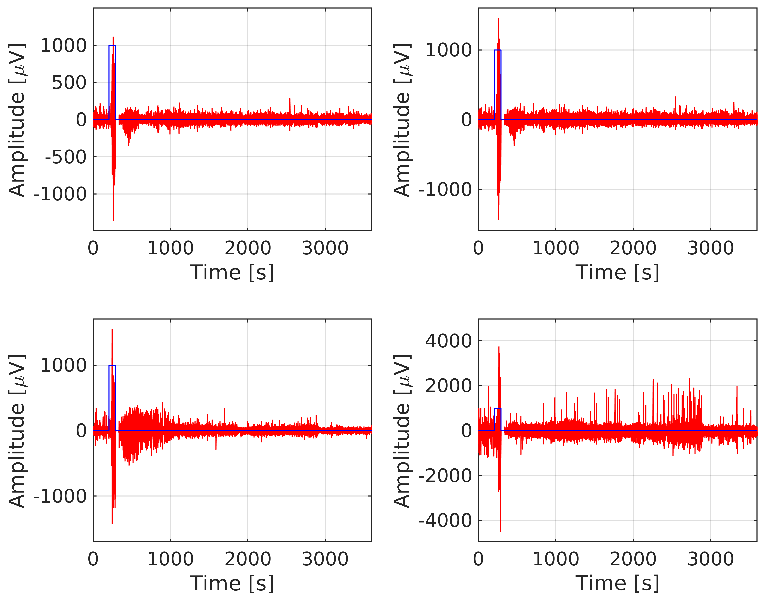
\includegraphics{./plots/iEEG_230_02_8_9_37_50.pdf}}
	\end{center}
	\caption{Preprocessed iEEG signals recorder by 4 electrodes out of 66, for second patient in 230th hour with marked seizure. Electrodes from left to right are 8, 9, 37, 50}

	\label{fig:iEEG_230_02_8_9_37_50}
\end{figure}

\begin{figure}[H]
	\begin{center}
		\scalebox{1.}{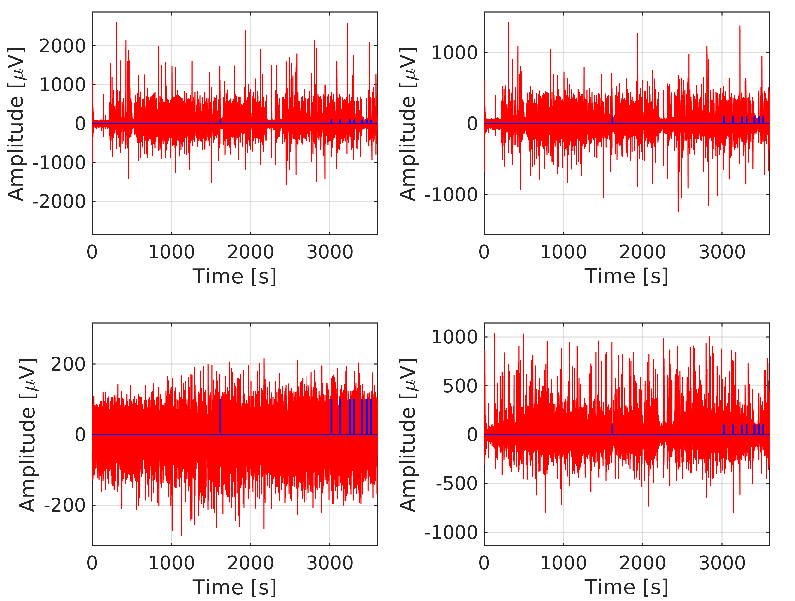
\includegraphics{./plots/iEEG_18_08_8_9_37_50.pdf}}
	\end{center}
	\caption{Preprocessed iEEG signals recorder by 4 electrodes out of 61, for 8th patient in 18th hour with marked seizures. Electrodes from left to right are 8, 9, 37, 50. 8 seizures recorded.}

	\label{fig:iEEG_18_08_8_9_37_50}
\end{figure}

\section{LBP patterns}
\subsection{2 dimensional LBP}
Local binary patterns (\verb|LBP|) have been used extensively in 2-D image processing and texture classification. Their ability to expose texture changes, toleration against illumination changes and computational simplicity make them powerful technique for a real-time image analyses \cite{lbp_facial}. The idea is fallowing. Divide an image into for instances 16x16 pixel size windows. Consequently for every pixel take for example 8 surrounding neighbour pixels. If the centre pixel has a greater value than his particular neighbour assign to that pixel 0 otherwise 1. Finally for every pixel with value 1 calculate $2^p$ and summarise every neighbour pixel with computed in that way value, $p$ is a pixel number counted for example clockwise. Described procedure is presented on the \figurename{} \ref{fig:LBP_2_D}.

\begin{figure}[H]
	\begin{center}
		\scalebox{.78}{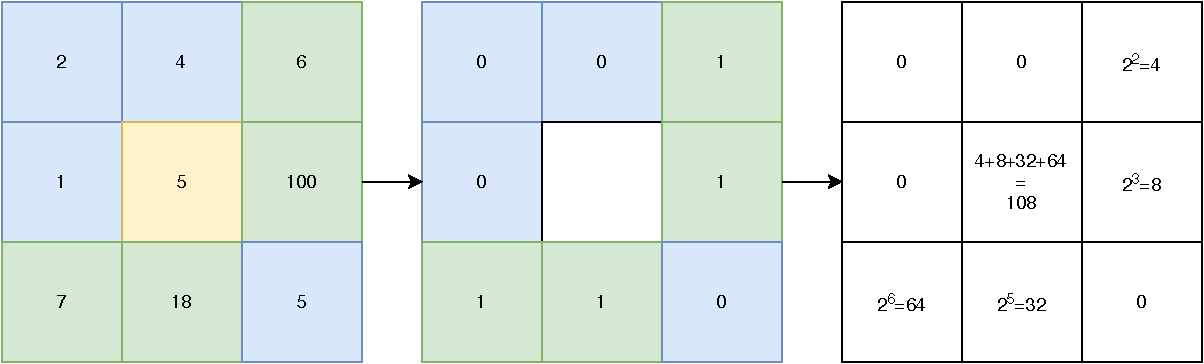
\includegraphics{./pictures/lbp_2_d.pdf}}
	\end{center}
	\caption{Exemplary local binary pattern for a part of 2D image.}

	\label{fig:LBP_2_D}
\end{figure}
In a formal way \verb|LBP| can be written as \ref{eq:lbp} where $p$ stands for pixel number, P number of surrounding pixels, in this example 8 and $\mathbf{1}$ is the Heaviside step function which transforms the difference between centre pixel $g_\mathrm{c}$ and neighbour $g_p$ into binary code.
\begin{equation} \label{eq:lbp}
\begin{aligned}
\text{LBP}(g_\mathrm{c}, \mathrm{P})=\sum_{p=0}^{\mathrm{P}-1} 2^p\mathbf{1}(g_p-g_\mathrm{c})
\end{aligned}
\end{equation}
When the \verb|LBP| code is calculated for every pixel in the window, the window can be approximated by the distribution of \verb|LBP| codes as a histogram. For 16x16 pixels window the histogram have 256 \verb|LBP| codes spread across $2^8-1$ values, which are number of
bins. Every \verb|LBP| value is counted and added to the group of the same \verb|LBP| value. Formal representation of an \verb|LBP| histogram is given by \ref{eq:histogram}. N stands for bins number which here is $2^8-1$, P is an \verb|LBP| length here 8, M represents a window size here 16x16, what gives 256 values where each \verb|ith| is the centre pixel and $\delta(a,b)$ is the Kronecker delta function.
\begin{equation} \label{eq:histogram}
\begin{aligned}
\mathrm{H}_{k\in[0, \mathrm{N}-1]}(\mathrm{M}, \mathrm{P}) = \sum_{i=0}^{\mathrm{M}-1} \delta(\mathrm{LBP}(i, \mathrm{P}), k)
\end{aligned}
\end{equation}
When the histogram of every window is calculated, they are concatenated what gives a feature vector for entire image \cite{lbp_facial}.
\subsection{1 dimensional LBP}
2 dimensional \verb|LBP| algorithm can be adapted into 1 dimensional space, thereby yielding possibility of taking advantage by signal processing. Several algorithms regarding \verb|iEEG| signals have already incorporated 1D local binary patterns with a great success for Alzheimer disease \cite{alzheimer} or epilepsy detection \cite{epilepsy_short},\cite{laelaps_long}. Rules applied to 2 dimensional space can be utilised by 1 dimensional \verb|LBP| analogously. \figurename{} \ref{fig:LBP_1_D} shows the path of \verb|LBP| code creation. It is worth noting that the way of computation varies between publications, namely some of them includes the centre point into binomial weights (power of 2) some of them not \cite{alzheimer}, \cite{lbp}. In this paper binomial weight is incorporated for the centre point. In addition in the \verb|LBP| length the centre point is not counted, what means the length of local binary pattern from \figurename{} \ref{fig:LBP_1_D} is 6 instead of 7.

\begin{figure}[H]
	\begin{center}
		\scalebox{.78}{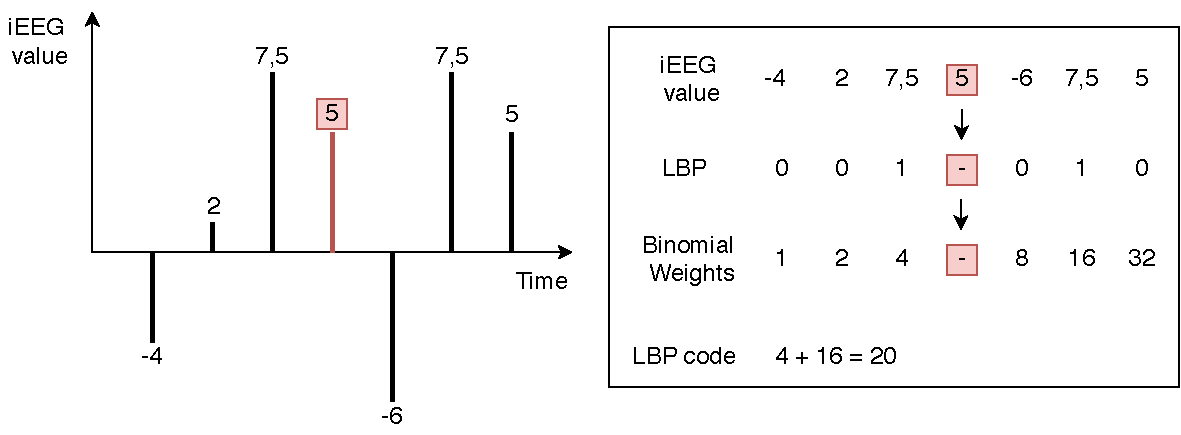
\includegraphics{./pictures/lbp_1_d.pdf}}
	\end{center}
	\caption{Exemplary local binary pattern for a part of iEEG signal.}

	\label{fig:LBP_1_D}
\end{figure}

The formula of one dimensional local binary pattern as well as the histogram is similar to \ref{eq:lbp} and \ref{eq:histogram}. The only difference is in the way of treatment $g_\mathrm{c}$ and $g_p$. For two dimensions these were pixels, here they are samples. In addition $\mathrm{M}$ value as a window size now is the part of \verb|iEEG| signal, for example 512 samples. When the histograms of multiple windows are computed they are juxtaposed one next to the another what results in the \figurename{} \ref{fig:histograms_1}. Each figure contains 86 histograms. Left one presents ictal stage whereas right one first 86 seconds of \verb|iEEG| measurement -- interictal stage. There is a huge resemblance between both figures, nonetheless some differences can be observed. Major one is in the \verb|LBP| value 8 -- during the seizure the amount of them was considerably bigger.

\begin{figure}[H]
	\begin{center}
		\scalebox{.58}{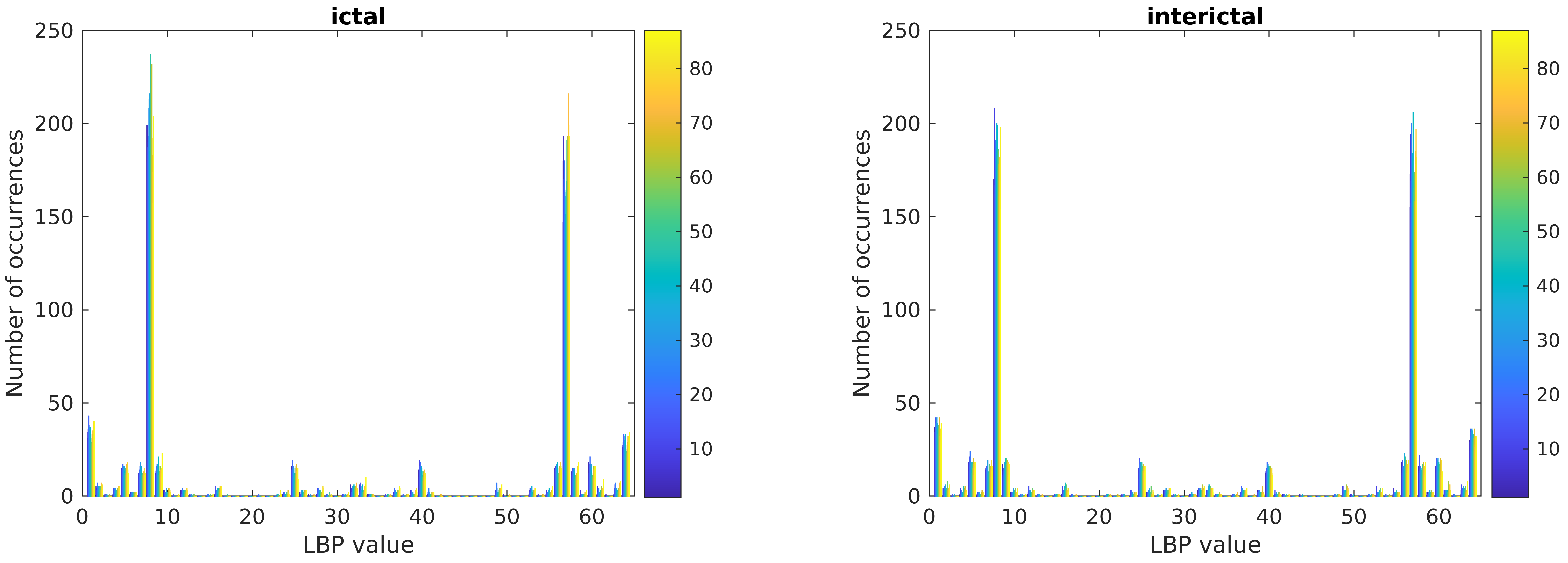
\includegraphics{./plots/histograms_6_230_02_8.pdf}}
	\end{center}
	\caption{86 histograms of window 512 samples (1 second) and LBP length 6 for the second patient in 230th hour and electrode number 5. On the left ictal state, interictal on the right}

	\label{fig:histograms_1}
\end{figure}
\figurename{} \ref{fig:histograms_2} contains histograms for the same period, patient and electrode, but with \verb|LBP| length 4 instead of 6. Similarly there is one significant major between two stages, this time in the amount of \verb|LBP| value 4. It is worth to remark, that histograms of Alzheimer cases have similar appearance \cite{alzheimer}. 
\begin{figure}[H]
	\begin{center}
		\scalebox{.58}{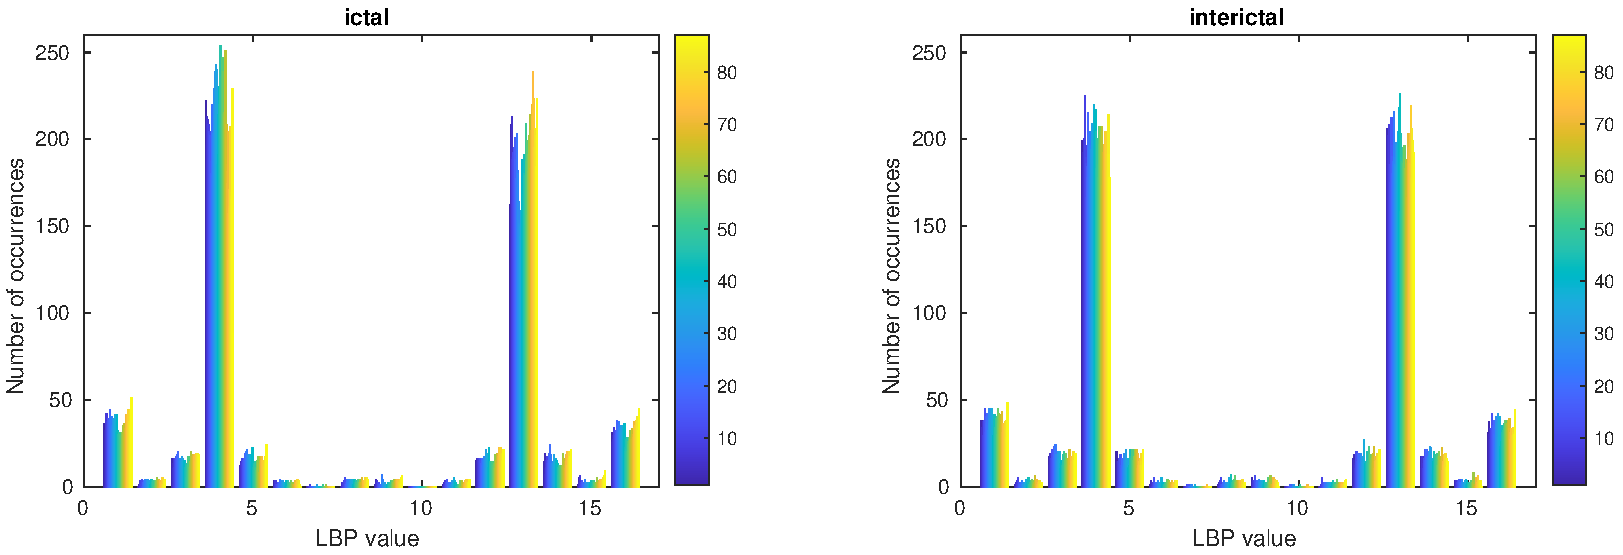
\includegraphics{./plots/histograms_4_230_02_8.pdf}}
	\end{center}
	\caption{86 histograms of window 512 samples (1 second) and LBP length 4 for the second patient in 230th hour and electrode number 5. On the left ictal state, interictal on the right}

	\label{fig:histograms_2}
\end{figure}
\paragraph{LBP implementation}
1 dimensional local binary patterns for a need of \verb|iEEG| processing are implemented in \verb|MATLAB|. The following function calculates \verb|LBP| and histograms for the given window and \verb|LBP| length.
\begin{lstlisting}[style=custommatlab,frame=single]
function [histogram_values, lbp_values] = calculate_histogram(y, P)
% P is even like 8 or 6
% y is a part of the signal numel(y) should be > 2^P, like 512 for LBP length 6
    P_2 = P/2; N =numel(y);
    % vector with content for example for P=3: [0 0 0 128 3 15 36 .. 0 0 0]
    lbp_values = zeros(1, N); 
    
    % amount of possible lbp values for example 2^8=256
    bins_number = 2^P;
    
    % in histogram_values on X axis 0 ... 256 and on Y number of occurrences
    % for example lbp_value = 3 occurred 6 times so on Y 6 on X 3
    histogram_values = zeros(1, bins_number);
    
    % for k=3 -> [1,2,4,0,16,32,64] 

    binomial_weights=zeros(1, P+1);
    for i=1:P_2 % first half
        binomial_weights(i)=2^(i-1);
    end
    % P+1 is a middle value -> thresholds in binomial_weights is 0
    for i=(P_2+2):(P+1) % second half
        binomial_weights(i)=2^(i-2);
    end

    for i=P_2+1:N-P_2 % first P/2 and last P/2 not counted
        lbp_vector=y(i-P_2:i+P_2); % size P+1, so with threshold value

        for j=1:P+1 % loop through every element in a window
            if lbp_vector(j) >= y(i) % i element is 1 in binary vector
                lbp_values(i) = lbp_values(i) + binomial_weights(j);
            end
        end
        histogram_values(lbp_values(i)+1) = histogram_values(lbp_values(i)+1) + 1;
    end
    %  number of omitted elements are added to zero occurrences
    histogram_values(1) = histogram_values(1) + P;
end
\end{lstlisting}
\begingroup
\renewcommand{\cleardoublepage}{}
\renewcommand{\clearpage}{}
\chapter{Neural Network}
\endgroup

There are several challenges for neural network which are necessary to mention. First of all neural network has to be capable of judgement if within particular period there was a seizure or not. Secondly the faster detection is, the better outcome for the potential exploitation of the seizure awareness, thereby possibly rendering seizures suppression. Neural network should not signalise seizure if in the reality the seizure does not occurred. In the worse case scenario device which takes an advantage of artificial intelligence would apply signals to the brain if they are not needed. One can say that there should not be any false alarms. All of mentioned requirements and challenges indicates that the neural network ought to be very well trained. The following chapter presents results of a deep feed forward neural network exploitation in the seizures detection basing both on preprocessed and raw \verb|iEEG| signals. Several multilayer perceptron configurations, that is different amount of nodes and hidden layers were tested and compared. In order to simplify future development of the project, namely \verb|VHDL| implementation of the neural network, the process of thinking (feedforward) was written in pure \verb|Python| without any high level libraries like \verb|NumPy|, \verb|PyTorch| or \verb|Tensorflow|. However the training was simplified and outsourced to the \verb|Tensorflow| in version 2. Weights and biases from the trained multilayer perceptron can be exported and utilised in the \verb|VHLD| or any other different technology. In the implementation the training reinforcement is supplied only for one hidden layer configuration (check Appendix \ref{ch:back}).

\section{Feedforward neural network}
Feedforward neural network is a multilayer perceptron with several hidden layers extensively used in machine learning along with deep convolutional neural networks and recurrent neural networks. The forward pass, so the process of thinking is relatively simple and performance effective. The \figurename{} \ref{fig:feedforward} shows deep feedforward neural network with multiple inputs and one output. In the feedforward process all inputs are multiplied by weights in the connection with the first hidden node what results in the net input $z_1[0]=i[0]w_1[0][0]+i[1]w_1[1][0]+\dots+i[k]w_1[k][0] + b_1[0]$. Subsequently the net input $z$ is applied to the activation function. The process is performed for every node in every hidden and output layer, where output from the particular node is an input of the next node. It is worth noting that the number of nodes in the hidden layers not necessarily has to be equal. Formal process of the feedforward pass for particular node is written in \ref{eq:histogram}, where $f_k$ represents activation function for the layer $k$ which is either \verb|ReLU| for hidden layers or \verb|sigmoid| for the output one. Rectified linear unit (\verb|ReLU|) has an advantage over \verb|sigmoid| function used in the output layer, because it does not have vanishing gradient, which prevents neural network from efficient learning. In fact \verb|ReLU| has the constant gradient. \verb|Sigmoid| activation function is given by \ref{eq:sigmoid}, whereas \verb|ReLU| by \ref{eq:ReLU}.

\begin{equation} \label{eq:feedforward}
\begin{aligned}
    z_k[0]&=n_{k-1}[0]w_k[0][0]+n_{k-1}[1]w_k[1][0]+\dots+n_{k-1}[m]w_k[m][0] + b_k[0] \\
    n_k[0]&=f_k(z_k[0]) \\
\end{aligned}
\end{equation}

\begin{equation} \label{eq:sigmoid}
f(z)=\frac{1}{1-e^{-x}}
\end{equation}

\begin{equation} \label{eq:ReLU}
f(z)=max(0, z)
\end{equation}

\begin{figure}[H]
	\begin{center}
		\scalebox{.6}{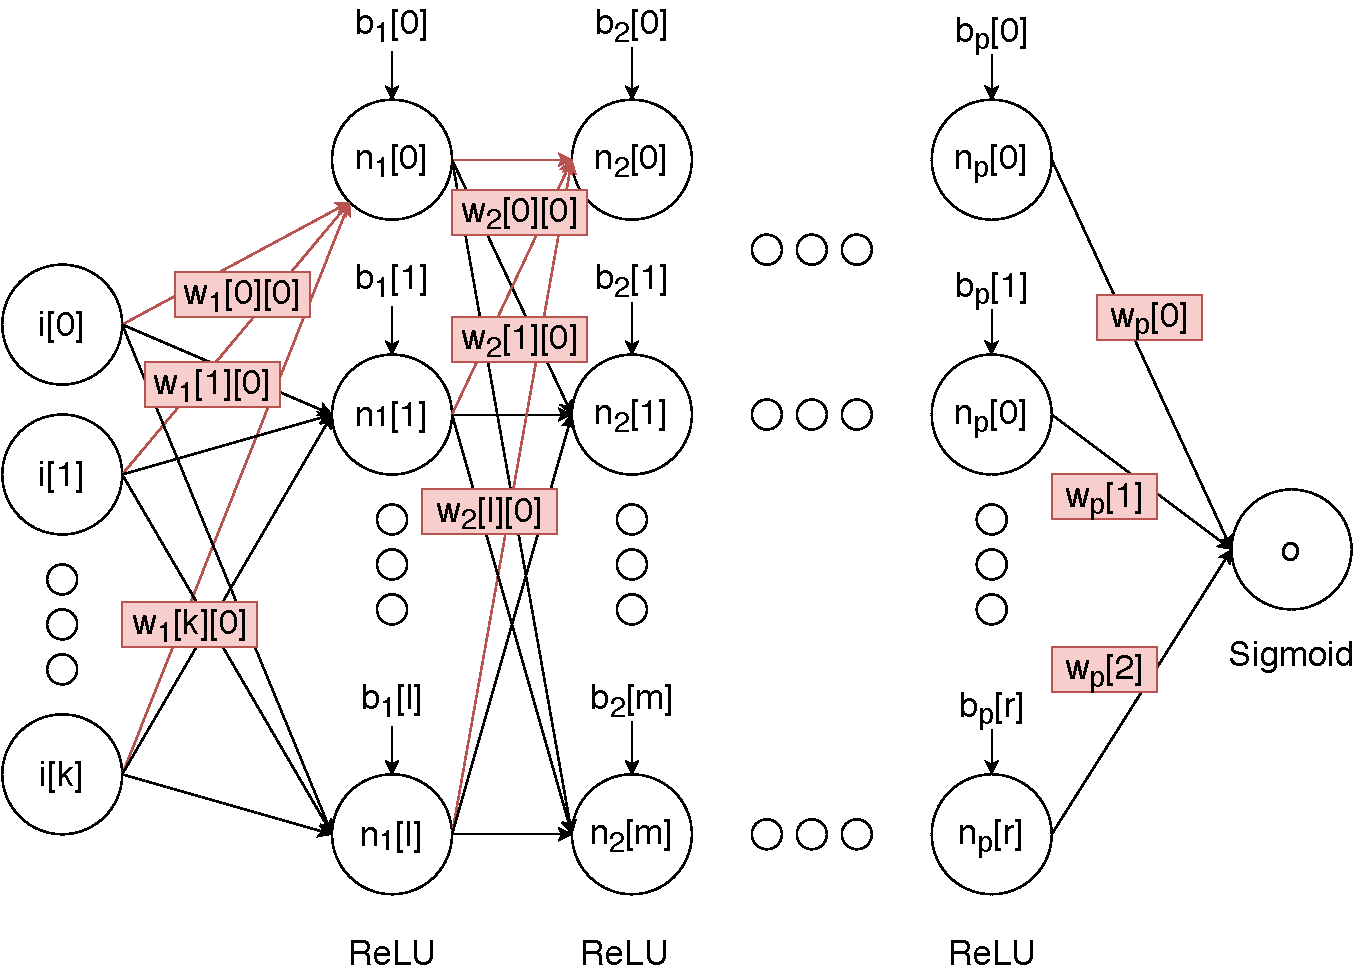
\includegraphics{./pictures/feedforward.pdf}}
	\end{center}
	\caption{Feedforward neural network with multiple inputs and one output. On the bottom of every layer, activation function was presented.}

	\label{fig:feedforward}
\end{figure}
The implementation of the feedforward pass is presented on the following listing. This function is invoked for every hidden layer and the output layer. The result of particular layer is passed to the consecutive one.
\begin{minted}[frame=single, linenos]{python}
def feedForward(self, inputs, weights_matrix, biases, activationFunction):
    input_length  = len(weights_matrix)
    output_length = len(weights_matrix[0])
    x = inputs
    y = []
    z = [] # without activation
    
    for o in range(0, output_length): # calculate each output in order
        y.append(0);
        z.append(0);
        for i in range(0, input_length):
            y[o] += weights_matrix[i][o]*x[i]
    
        z[o] = y[o] + biases[o]
        y[o] = activationFunction(z[o])
        
    return y, z
\end{minted}

\section{Training process}
Training was performed using \verb|Tensorflow| library in the version of \verb|2.2|. Time of training varies between dozen minutes to even several hours, depending on the amount of epochs, nodes in the particular layer and the layers itself. Neural network is fully connected. As a lost function binary cross entropy was used, it is given by the formula \ref{eq:bce}, where $y_a$ and $y_d$ are the actual outputs of the neural network respectively and $L$ is the loss function.
\begin{equation} \label{eq:bce}
L(y_a,y_t)=-[y_alog(y_d)+(1-y_a)log(1-y_d)]
\end{equation}
The training process starts with the model definition, goes through the training itself and finally finishes on the model saving as well as the weights and biases in the proper format. These weights and biases are then consumed by the custom \verb|Feedforward| class and used in the prediction process. The following listing shows the training implementation for 4 hidden layers. First hidden layer has 200 nodes, second 100 and so on.
\begin{minted}[frame=single, linenos]{python}
def createModel(self):
    self.model = keras.Sequential([
                 keras.layers.Dense(200, activation="relu"),
                 keras.layers.Dense(100, activation="relu"), 
                 keras.layers.Dense(50, activation="relu"),
                 keras.layers.Dense(20, activation="relu"),
                 keras.layers.Dense(1, activation="sigmoid")
        ])
    self.model.compile(optimizer="adam", loss="binary_crossentropy", 
        metrics=["accuracy"])

def trainModel(self, epochs_num, save=True):
    self.model.fit(self.train_data, self.train_labels, epochs=epochs_num)
    test_loss, test_acc = self.model.evaluate(self.test_data, self.test_labels)
\end{minted}
Both training and test data are generated in the \verb|csv| format by \verb|MATLAB|. They representation varies on the experiment and can be a group of some \verb|iEEG| following samples for example 512 or \verb|LBP| histogram values. The expected value always is a desired prediction which ranges between 0 and 1, where 0 stands for no seizure, 1 for the seizure. Technically it is a probability of the seizure occurrence.

\begingroup
\renewcommand{\cleardoublepage}{}
\renewcommand{\clearpage}{}
\chapter{Experiments}
\endgroup
Training and testing is done for the patient 2, in whom clearly visible seizure occurred in 230th and 233th hour what is presented on the \figurename{} \ref{fig:iEEG_230_233_02_8}. Several tests with \verb|LBP| patterns, raw data and \verb|FIR| filter were performed. The methodology is the following. First test and train data are generated using \verb|MATLAB| were depending on the test every column represents the amount of occurrences of particular \verb|LBP| pattern (histograms), part of a raw signal or part of the signal passed through the \verb|FIR| filter. As a last column the desired prediction is placed, which is value either 1 or 0 if the seizure was observed or was not by the specialist in the particular moment. Every train and test file contains 3600 rows, where each row contains 1 second of normalised data. Several variants of feedforward neural network with different amount of epochs during training process were tested. After the training, train data are passed through the network to judge the function adjustment and of course test data to check the prediction. Both processes are juxtaposed next to each other on the figures in 2 columns.

\begin{figure}[H]
	\begin{center}
		\scalebox{.58}{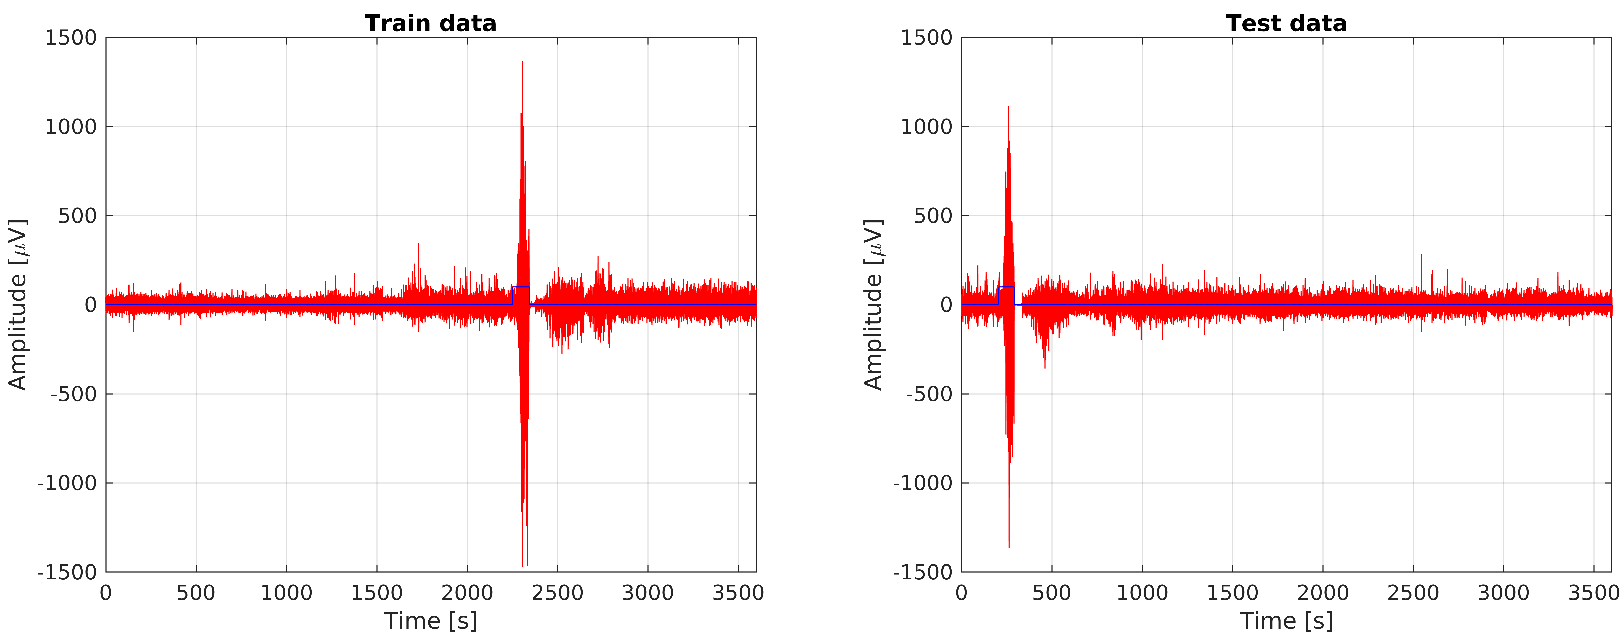
\includegraphics{./plots/iEEG_230_233_02_8.pdf}}
	\end{center}
	\caption{Training (233th hour) and testing (230th hour) data for the patient 2, electrode 8th with marked seizure.}

	\label{fig:iEEG_230_233_02_8}
\end{figure}

\section{LBP}
\verb|LBP| length of 4 and 6 was tested. Test and training data were scaled to the values between 0 and 1 where 1 represents upper bound common for the testing and training data.

\subsection{LBP Length 4}
\subsubsection{2 hidden layers}
\figurename{} \ref{fig:nn_lbp_2_hidden_16_50_40_1_1000_epochs} presents accuracy of the neural network with 16 inputs (\verb|LBP| length 4), 2 hidden layers with respectively 50 and 40 nodes and test of that network performed on the 230th hour. Training took around 2 minutes for 1000 epochs. 

\begin{figure}[H]
	\begin{center}
		\scalebox{.57}{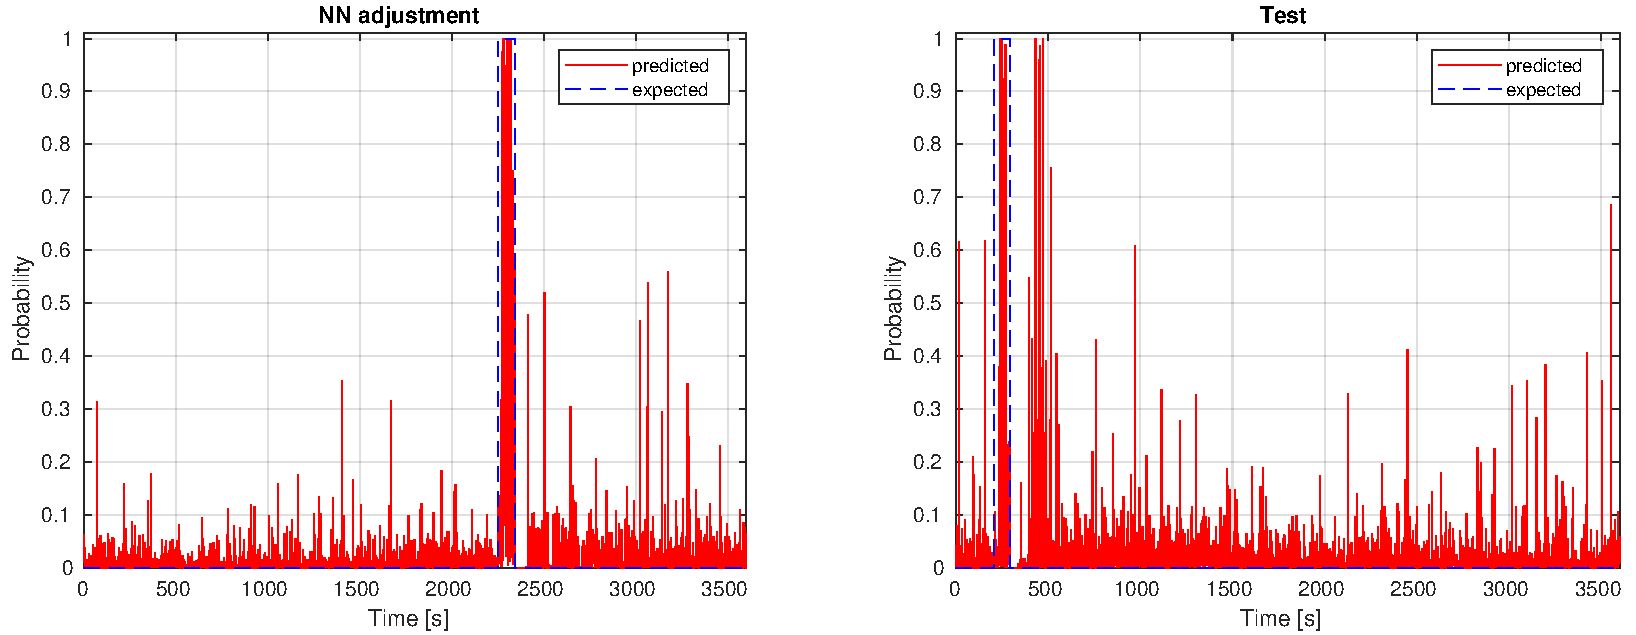
\includegraphics{./plots/nn_lbp_2_hidden_16_50_40_1_1000_epochs.pdf}}
	\end{center}
	\caption{On the left the neural network adjustment to the training data, on the right test. 16 inputs, number of nodes in 2 hidden layers are respectively 50, 40. Number of epochs 1000. Accuracy \num{0.9736111}}

	\label{fig:nn_lbp_2_hidden_16_50_40_1_1000_epochs}
\end{figure}
The accuracy of the model is low with poor adjustment to the expected value. In the test part there are many false alarms after the seizure. \figurename{} \ref{fig:nn_lbp_2_hidden_16_50_40_1_2000_epochs} shows exactly the same experiment results, but for 2000 epochs. Time of the training is 2 times longer and took 4 minutes. In spite of more epochs due to the overfitting the resutls are worse than for 1000 epochs.

\begin{figure}[H]
	\begin{center}
		\scalebox{.57}{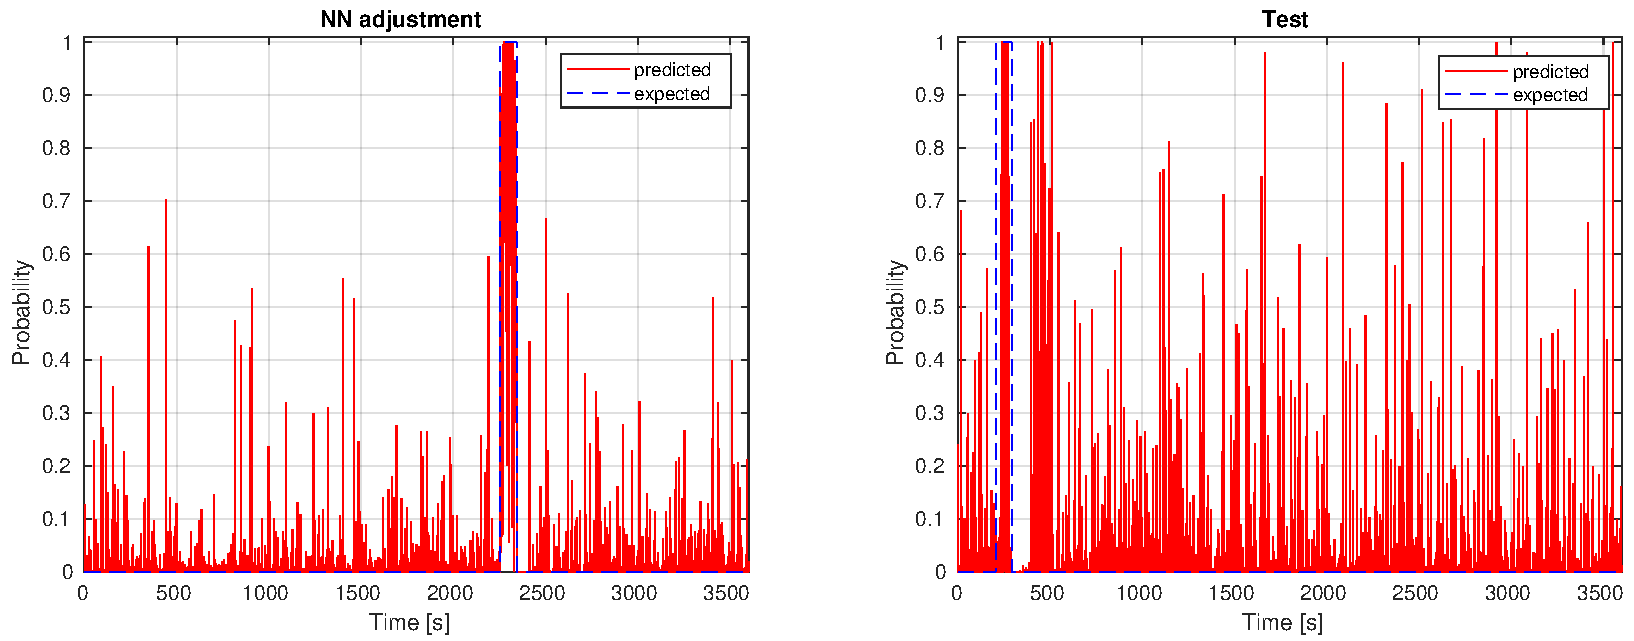
\includegraphics{./plots/nn_lbp_2_hidden_16_50_40_1_2000_epochs.pdf}}
	\end{center}
	\caption{On the left the neural network adjustment to the training data, on the right the test. 16 inputs, number of nodes in 2 hidden layers are respectively 50, 40. Number of epochs 2000. Accuracy \num{0.966389}}

	\label{fig:nn_lbp_2_hidden_16_50_40_1_2000_epochs}
\end{figure}

\subsubsection{3 hidden layers}
Next experiment was performed for 3 hidden layers. First hidden layer has 100 nodes, second 60 and third one 40 nodes. The best result attained throughout the experiments is presented on the \figurename{} \ref{fig:nn_lbp_3_hidden_16_100_60_40_1_500_epochs}. Training was carried out 500 times, higher value resulted in bigger overfitting.

\begin{figure}[H]
	\begin{center}
		\scalebox{.57}{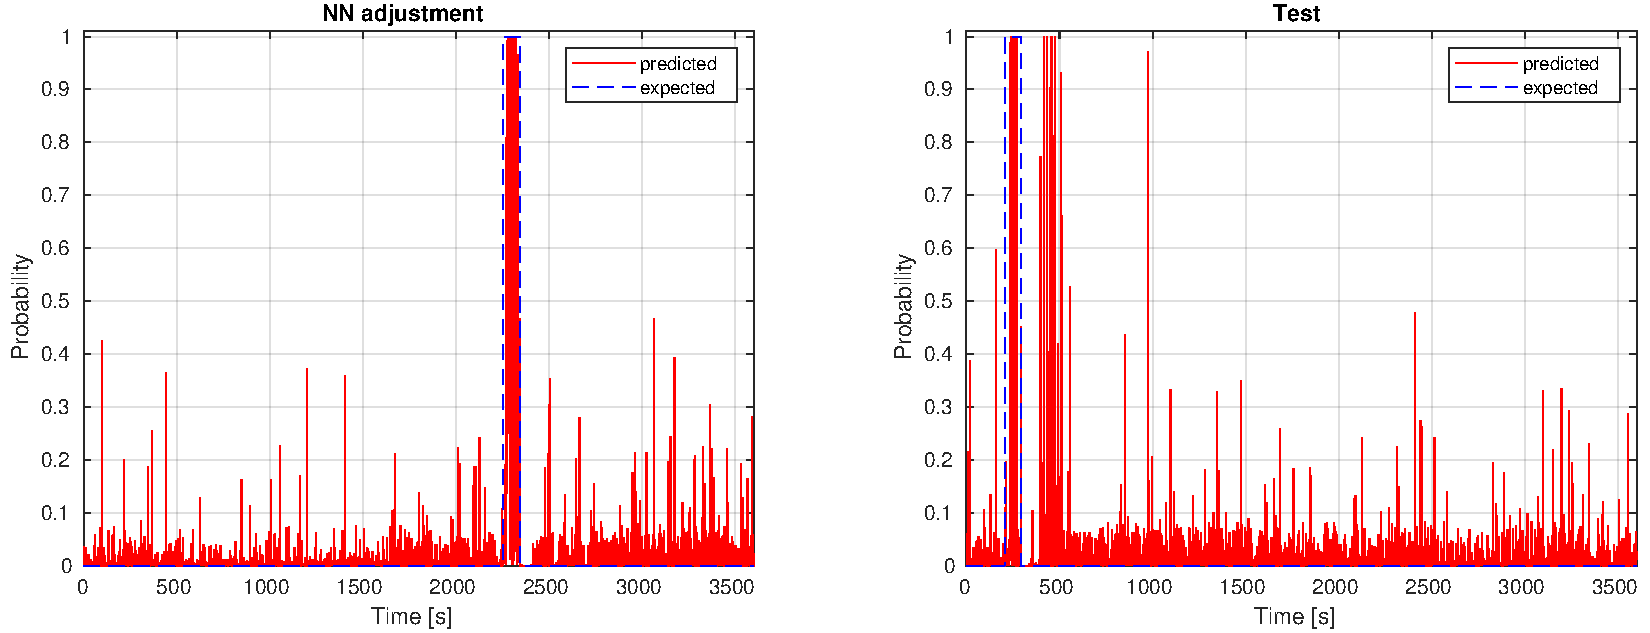
\includegraphics{./plots/nn_lbp_3_hidden_16_100_60_40_1_500_epochs.pdf}}
	\end{center}
	\caption{On the left the neural network adjustment to the training data, on the right the test. 16 inputs, number of nodes in 3 hidden layers are respectively 100, 60, 40. Number of epochs 500. Accuracy \num{0.976111}}

	\label{fig:nn_lbp_3_hidden_16_100_60_40_1_500_epochs}
\end{figure}

\subsubsection{4 hidden layers}

Finally 4 hidden layers were tested with the following amount of nodes: 200, 100, 50, 20. Unfortunately the result is not satisfactory. After many experiments with the \verb|LBP| length of 4, eliminating the false epilepsy alarm around 500 second was not successful. The performance of the network does not improve with the amount of nodes and layers. It is worth to mention that the process of thinking is significantly longer than for 3 and 2 layers. \figurename{} \ref{fig:nn_lbp_4_hidden_200_100_50_20_1_500_epochs} shows the testing and training result of 100 epochs for 4 layers perceptron.

\begin{figure}[H]
	\begin{center}
		\scalebox{.57}{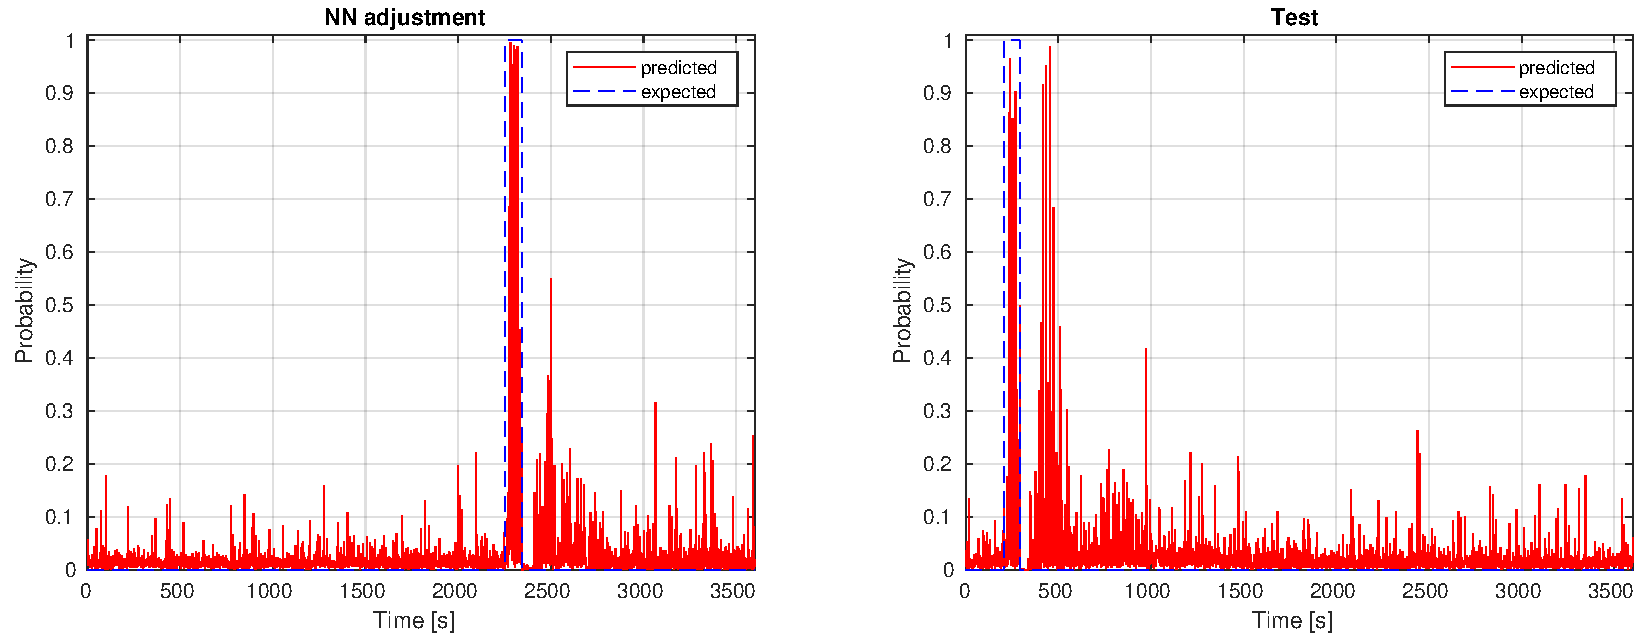
\includegraphics{./plots/nn_lbp_4_hidden_200_100_50_20_1_500_epochs.pdf}}
	\end{center}
	\caption{On the left the neural network adjustment to the training data, on the right test. 16 inputs, number of nodes in 4 hidden layers are respectively 200, 100, 50, 20. Number of epochs 100. Accuracy \num{0.9763888}}

	\label{fig:nn_lbp_4_hidden_200_100_50_20_1_500_epochs}
\end{figure}

\subsection{LBP Length 6}
After many consecutive experiments there was not any neural network configuration either from the number of layers, nodes or the number of epochs point of view. The best results were accomplished for 3 layers with the same amount of nodes in every layer, apart from the output. The result is showed on the \figurename{} \ref{fig:nn_lbp_3_hidden_64_64_64_64_1_100_epochs} 

\begin{figure}[H]
	\begin{center}
		\scalebox{.57}{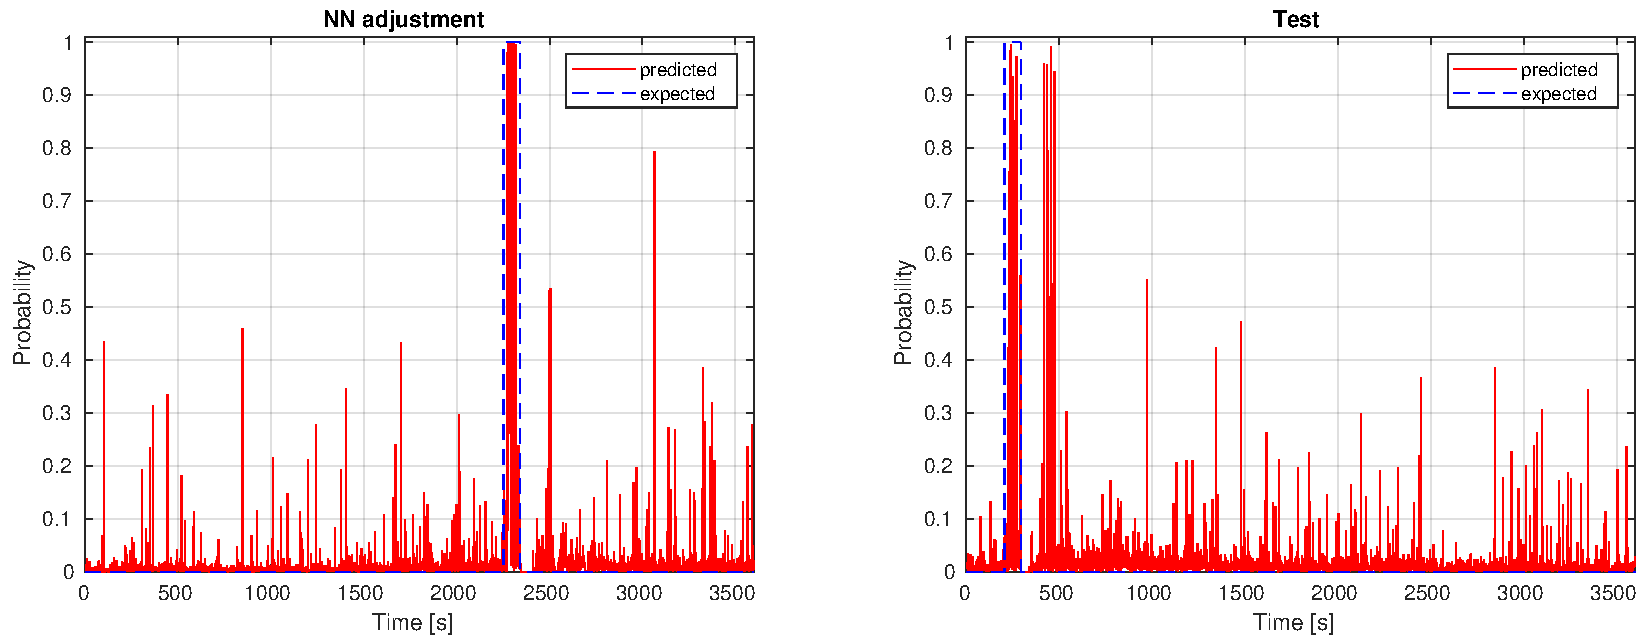
\includegraphics{./plots/nn_lbp_3_hidden_64_64_64_64_1_100_epochs.pdf}}
	\end{center}
	\caption{On the left the neural network adjustment to the training data, on the right test. 64 inputs, number of nodes in 3 hidden layers 64, 64, 64. Number of epochs 100. Accuracy \num{0.976666}}

	\label{fig:nn_lbp_3_hidden_64_64_64_64_1_100_epochs}
\end{figure}
\subsection{LBP summary}
Several configurations were tested regarding local binary patterns. Different amount of layers and nodes as well as epochs were thoroughly explored. It is extremely difficult to shed many of the false alarms, especially these right after the epilepsy. Nevertheless as it was pointed in the former research, local binary patterns were successfully exploited in the epilepsy and Alzheimer detection \cite{alzheimer}, \cite{epilepsy_short}, \cite{laelaps_long}. Taking this into account, the problems with detection presented in this paper may be caused by utilising only one electrode from the group of dozen. Second reason can be in the fact that histogram windows do not overlap one another. It is possible that the result would be different if adjacent windows had common part. However it would extend amount of samples from 3600 to 7200 for half a second overlap and so on resulting in the longer training. This should be investigated in the further research.  
\section{Raw data}
Next set of experiments regards raw digitised \verb|iEEG| samples. As in the local binary patterns the window was 512 samples, here similarly there are 512 samples, where every adjacent input receives one particular adjacent sample. In addition adjacent windows do not overlaps one another. First remarkable thing in these experiments is the time of feed forward pass and the back-propagation process which is much longer than for \verb|LBP|. The reason is in the weights amount between layers which increases exponentially with the nodes and layers number. 

\subsection{2 hidden layers}
At the beginning neural network with 2 hidden layers was tested with consecutive 400 and 40 nodes. The result is remarkable better than using local binary patterns. \figurename{} \ref{fig:nn_raw_2_hidden_512_400_40_1_1000_7000_10000_not_zoomed} shows 3 experiments with a different quantity of epochs. Starting with the first row it is 1000, 7000 and 10000 epochs. On the left side adjustment of the network to the training data is showed, on the right the prediction. The more epochs the better adjustment, but at some point at the price of overfitting, what is showed on the third row.

\begin{figure}[H]
	\begin{center}
		\scalebox{.57}{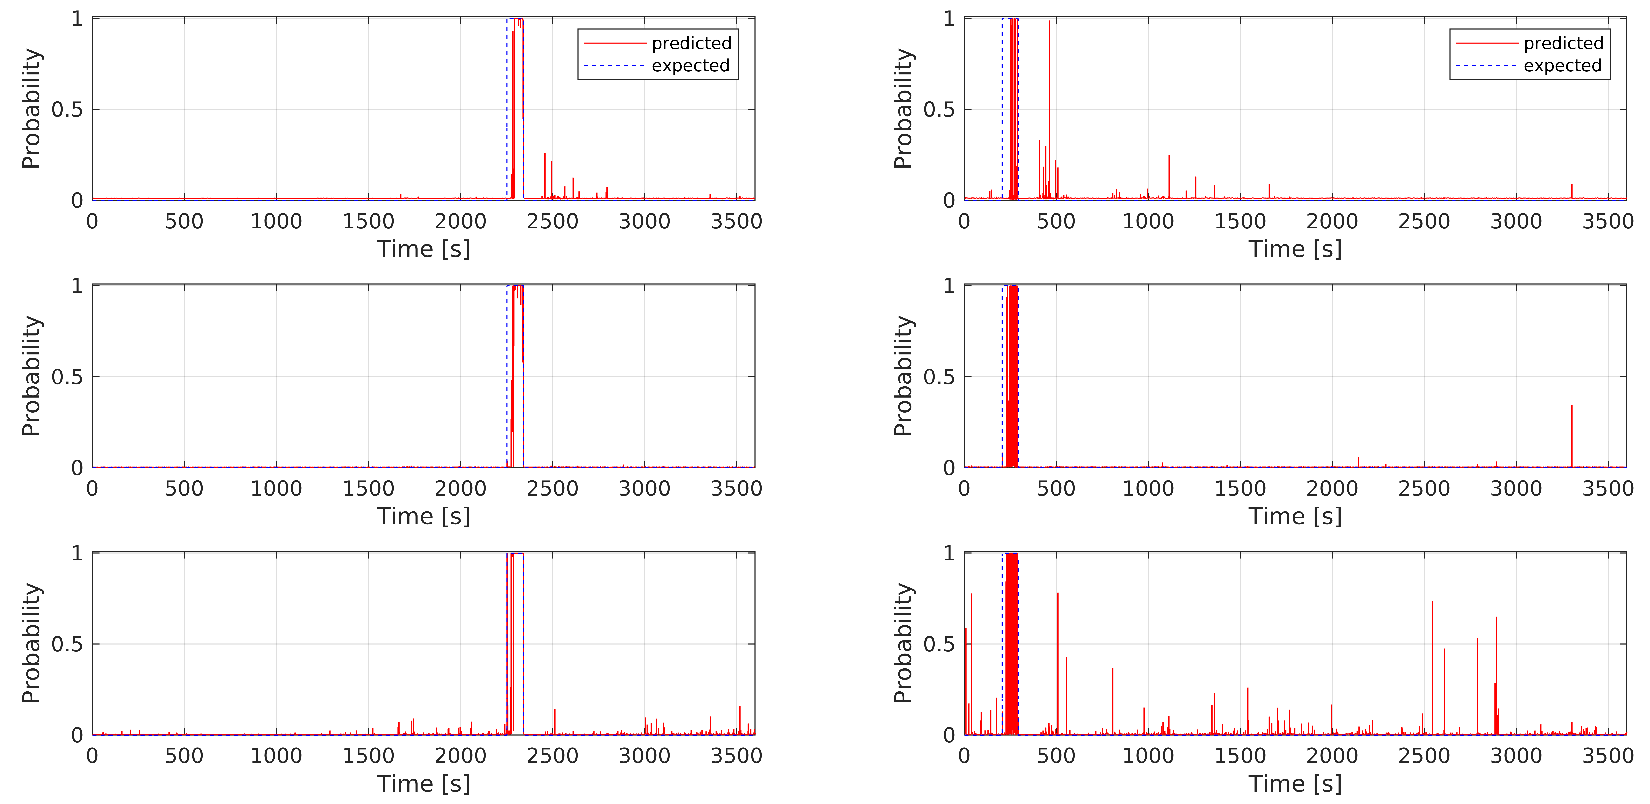
\includegraphics{./plots/nn_raw_2_hidden_512_400_40_1_1000_7000_10000_not_zoomed.pdf}}
	\end{center}
	\caption{3 experiments for 2 hidden layers multilayer perceptron. On the left network adjustment, on the right test. 512 inputs, number of nodes in 2 hidden layers 400, 40. Number of epochs in the particular raw is 1000, 7000, 10000 consecutively. Electrode 8.}

	\label{fig:nn_raw_2_hidden_512_400_40_1_1000_7000_10000_not_zoomed}
\end{figure}
The \figurename{} \ref{fig:nn_raw_2_hidden_512_400_40_1_1000_7000_10000} shows exactly the same experiments as \figurename{} \ref{fig:nn_raw_2_hidden_512_400_40_1_1000_7000_10000_not_zoomed} with zoomed seizure period. Red curve is supposed to very accurately fit the blue one, but instead there is a delay in the prediction around 30 seconds long for the second row, that is 7000 epochs experiment. Moreover the prediction jumps from 0 to 1 which is not what is expected. 

\begin{figure}[H]
	\begin{center}
		\scalebox{.57}{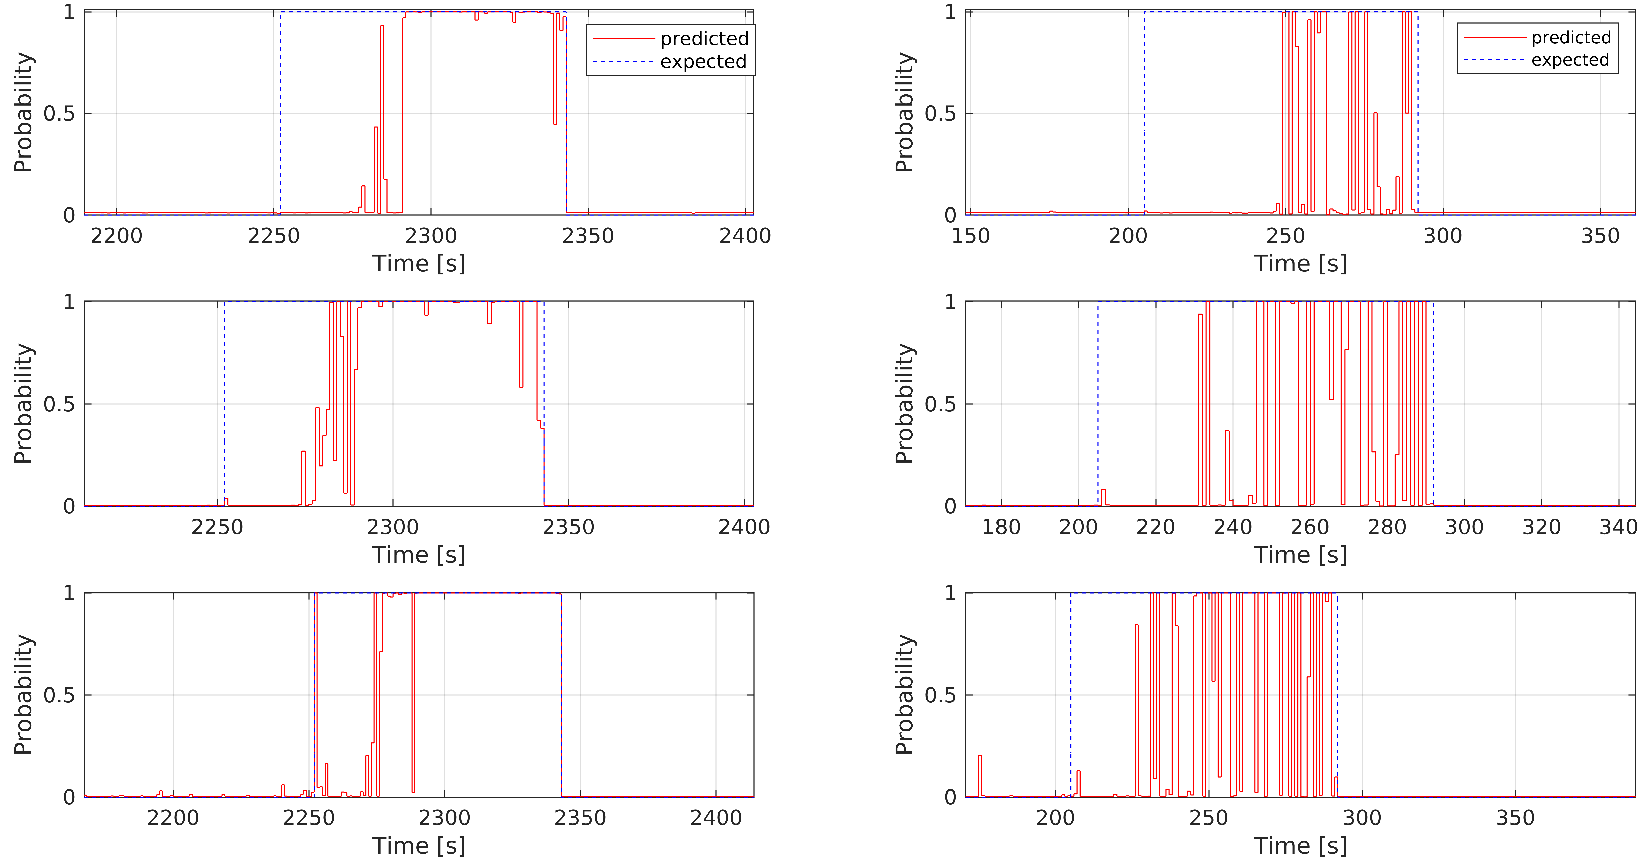
\includegraphics{./plots/nn_raw_2_hidden_512_400_40_1_1000_7000_10000.pdf}}
	\end{center}
	\caption{Zoomed experiment showed with 2 hidden layers. Delay can be observed as well as the prediction's jumps.}

	\label{fig:nn_raw_2_hidden_512_400_40_1_1000_7000_10000}
\end{figure}

\subsection{4 hidden layers}
Second tested neural network configuration was with 4 hidden layers, with consecutive number of nodes as 400, 300, 150 and 20. 
\begin{figure}[H]
	\begin{center}
		\scalebox{.57}{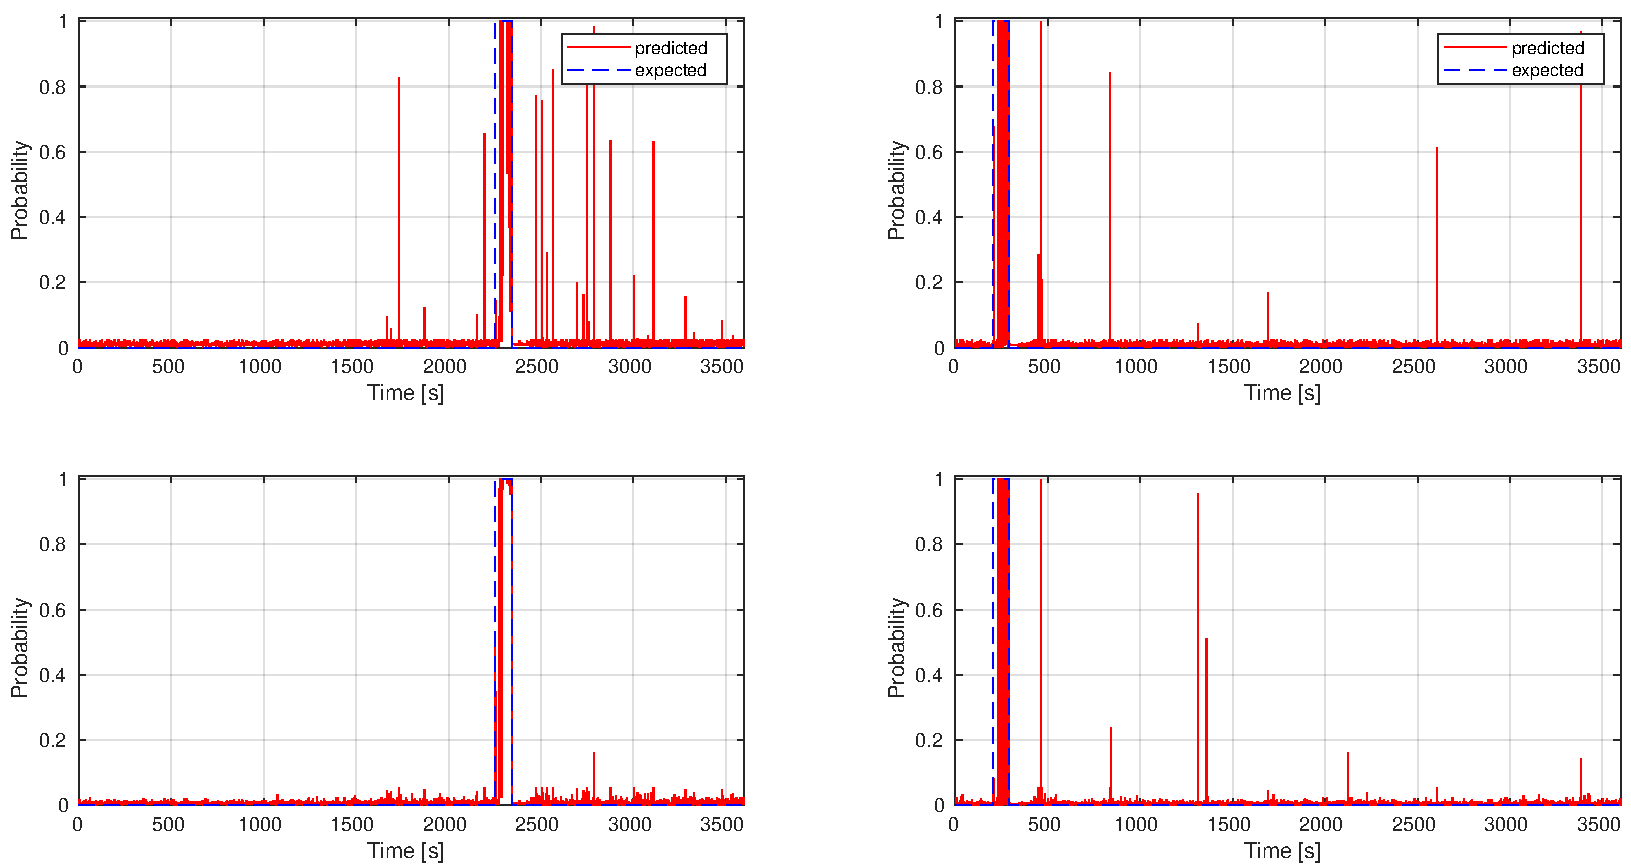
\includegraphics{./plots/nn_raw_4_hidden_512_400_300_150_20_1_30000_40000.pdf}}
	\end{center}
	\caption{2 experiments for 4 hidden layers multilayer perceptron. On the left network adjustment, on the right test. 512 inputs, number of nodes in 4 hidden layers 400, 300, 150, 20. Number of epochs in the particular raw is 30000 and 40000 consecutively.}

	\label{fig:nn_raw_4_hidden_512_400_300_150_20_1_30000_40000}
\end{figure}
On the \figurename{} \ref{fig:nn_raw_4_hidden_512_400_300_150_20_1_30000_40000}
the result of the performed experiments is presented. Second experiment is remarkably better from the adjustment point of view in the seizure time, however detection seems to be subject to fail, because of the several false alarms. In the next experiment the number of nodes in 4 layers was increased to 512, 400, 250 and 30.
\begin{figure}[H]
	\begin{center}
		\scalebox{.57}{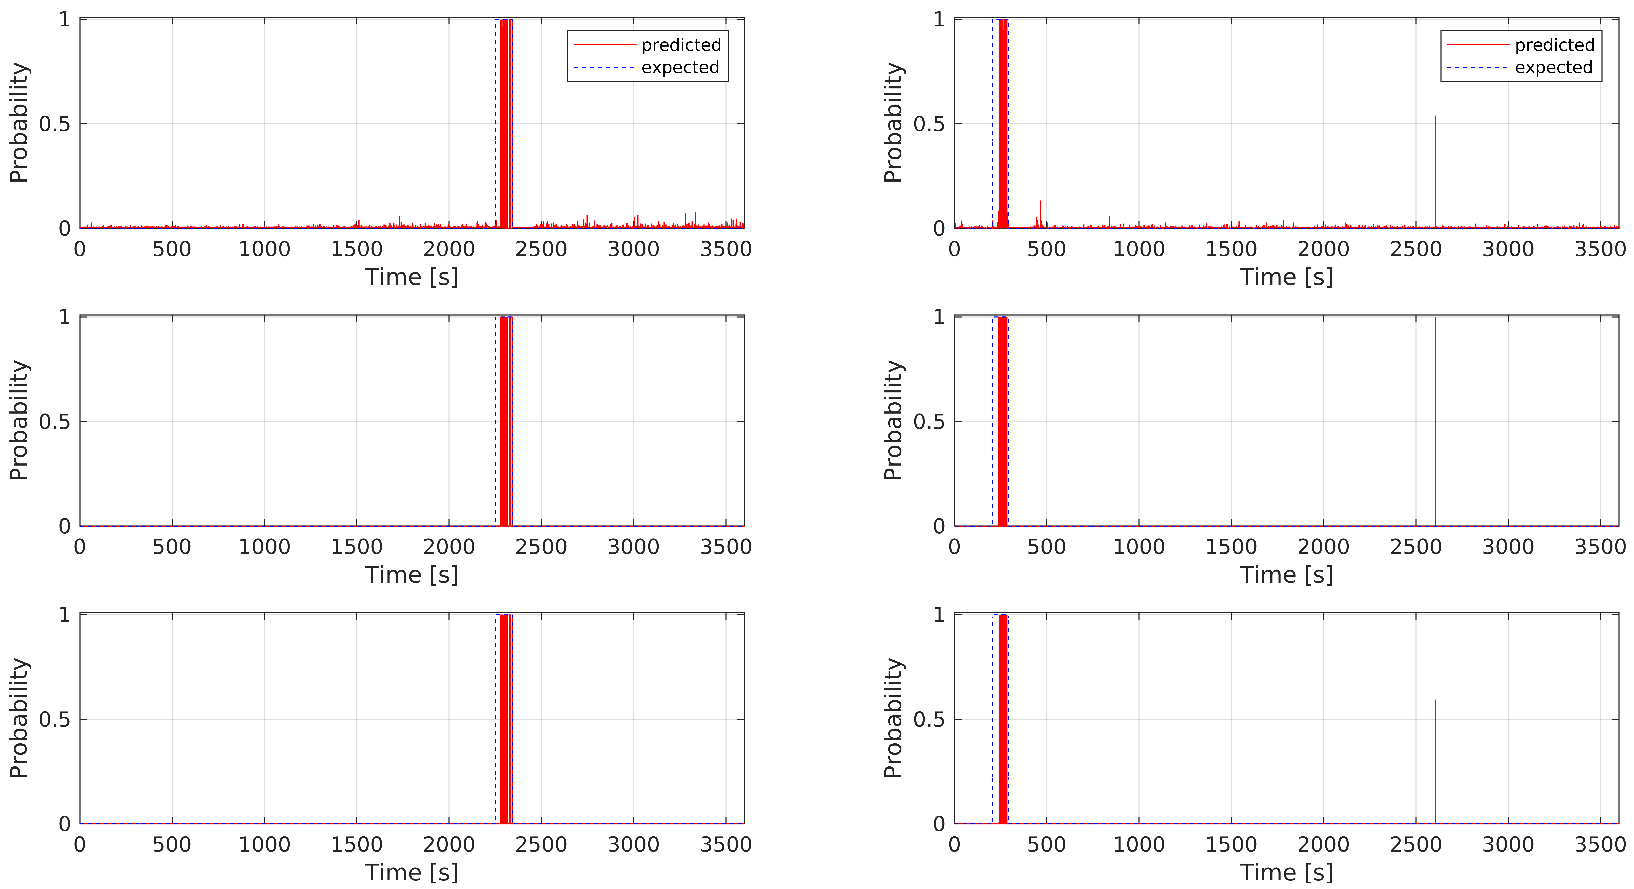
\includegraphics{./plots/nn_raw_4_hidden_512_400__250_30_1_5000_150000_20000.pdf}}
	\end{center}
	\caption{3 experiments for 4 hidden layers multilayer perceptron. On the left network adjustment, on the right test. 512 inputs, number of nodes in 4 hidden layers 512, 400, 250 and 30. Number of epochs in the particular raw is 5000, 15000, 20000 consecutively.}

	\label{fig:nn_raw_4_hidden_512_400__250_30_1_5000_150000_20000}
\end{figure}
\begin{figure}[H]
	\begin{center}
		\scalebox{.57}{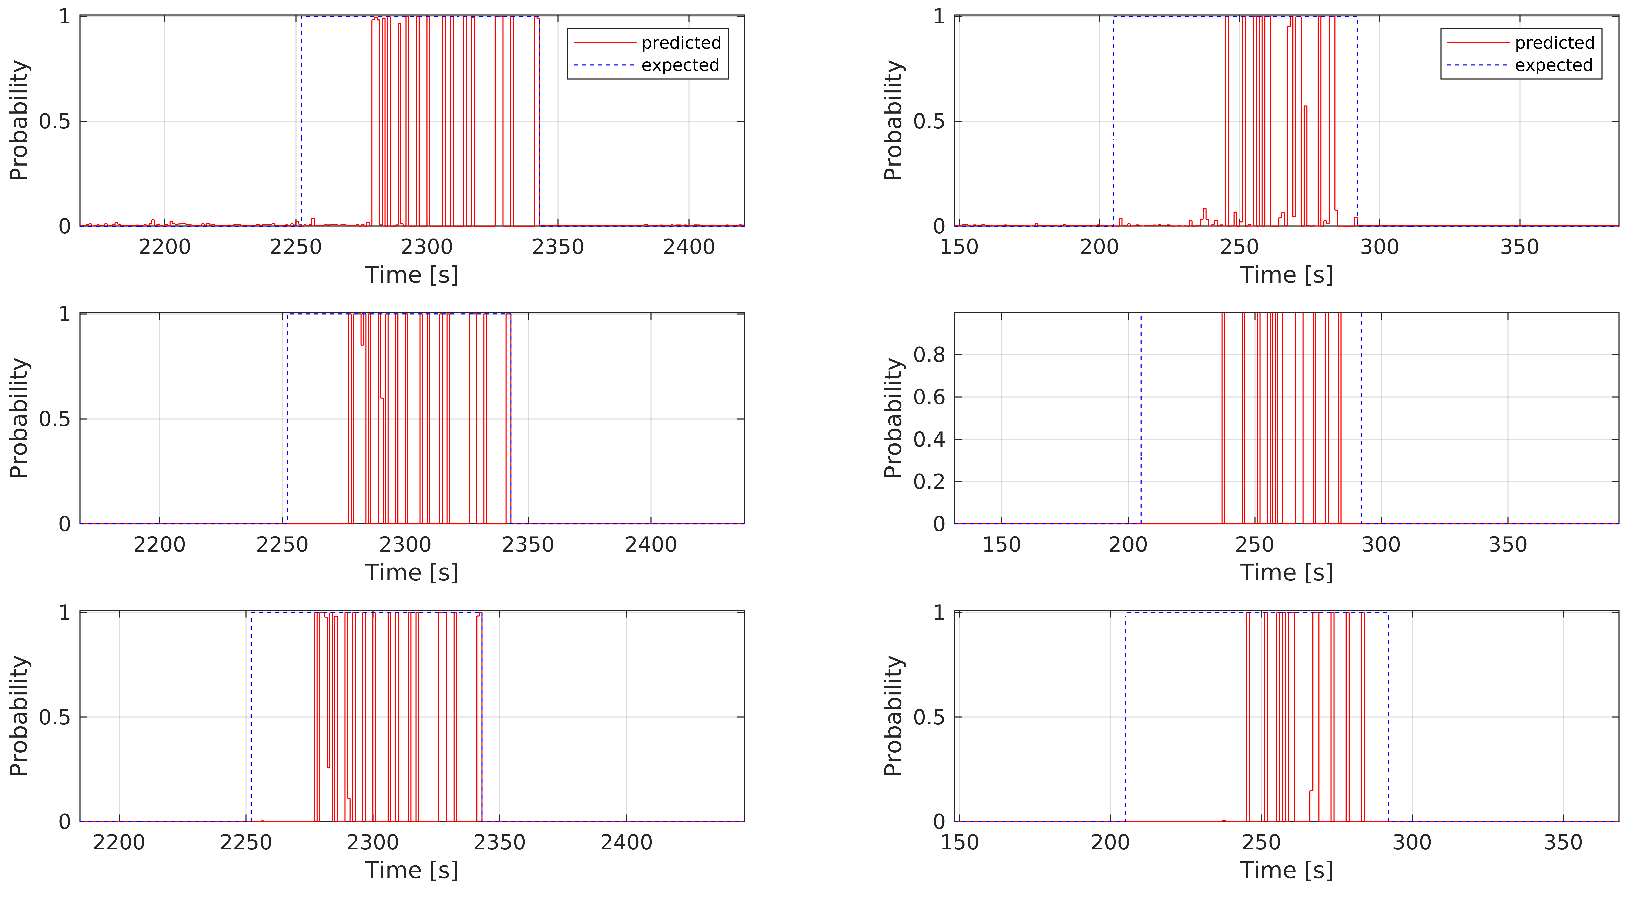
\includegraphics{./plots/nn_raw_4_hidden_512_400__250_30_1_5000_150000_20000_zoomed.pdf}}
	\end{center}
	\caption{Zoomed experiment with 4 hidden layers. Delay can be observed as well as the prediction's jumps, even bigger than for 2 layers. False alarms disappeared nonetheless.}

	\label{fig:nn_raw_4_hidden_512_400__250_30_1_5000_150000_20000_zoomed}
\end{figure}

\figurename{} \ref{fig:nn_raw_4_hidden_512_400__250_30_1_5000_150000_20000} shows 3 similar experiments as a \figurename{} \ref{fig:nn_raw_2_hidden_512_400_40_1_1000_7000_10000}, but this time with 5000, 10000 and 15000 epochs and 4 hidden layers. Seemingly after additional hidden layer the prediction as well as the neural network adjustment is better, but in the reality it happened only within interictal stage. During seizure phenomena as for 2 hidden layers occurred, namely prediction's jumps and delay, \figurename{} \ref{fig:nn_raw_4_hidden_512_400__250_30_1_5000_150000_20000_zoomed}. Moreover there is a false alarm around 2600th second for each experiment. 
Nevertheless the prediction is better comparing to the smaller number of nodes with the same amount of layers. False alarms were almost fully eliminated.
\section{Finite Impulse Response}
Finite Impulse Response, well known as a \verb|FIR| filter was applied for a need of an epilepsy detection in the last set of experiments of this paper. \verb|FIR| filter is extensively used in digital signal processing together with Infinite Impulse Response filter \verb|IIR|. Finite Input Response filter is described by the formula \ref{eq:FIR}, where $x[n]$ is an input signal, $y[n]$, \verb|FIR| output signal, N filter order and $b_i$ is a filter's coefficient.

\begin{equation} \label{eq:FIR}
y[n]=\sum_{i=0}^{\mathrm{N}} b_i x[n-i]
\end{equation}

The simple variant of the \verb|FIR| filter is moving-average filter, often used to smooth data \cite{fir_goerge_ellis}. In these example $b_i$ coefficients equal $\frac{1}{N+1}$, so intuitively it is a moving average of window N. These \verb|FIR| variant is used in the last experiment. Because of inputs normalisation, however the samples sum of the signal is not divided by the window's amount, in this variant the coefficients equal 1. The following listing shows the filter implementation in \verb|MATLAB|.
\begin{lstlisting}[style=custommatlab,frame=single]
N=fs; % window == 1 second
m=1;  % move by one sample
fir = zeros(1, samples_number);                  
for i = N:m:samples_number 
    fir(i) = mean(y(i-N+1 : i));
end
\end{lstlisting}
\figurename{} \ref{fig:fir_raw} shows the outcome of applying \verb|iEEG| signal to the \verb|FIR| filter. Two bottom plots present zoomed region around 205th second. \verb|FIR| smooth the signal, but rendering ictal and interictal periods more similar. 
\begin{figure}[H]
	\begin{center}
		\scalebox{.57}{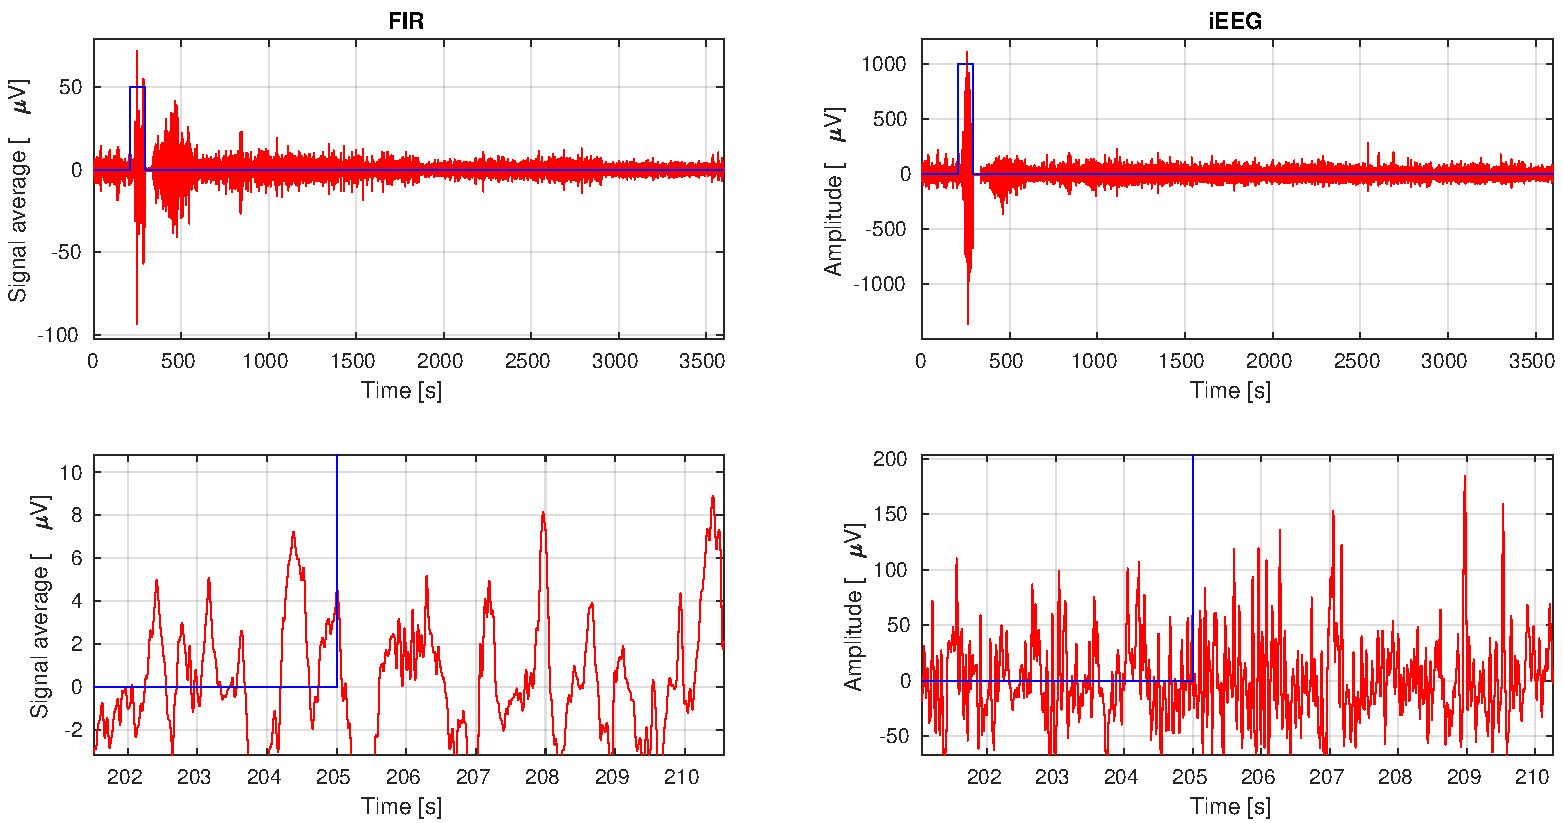
\includegraphics{./plots/fir_raw.pdf}}
	\end{center}
	\caption{FIR and raw iEEG comparison. FIR smooth the signal. Because of the average, ictal and interictal are more akin to each other.}

	\label{fig:fir_raw}
\end{figure}
\subsection{4 hidden layers}
Test was performed only for 4 hidden layers with 400, 300, 150 and 20 nodes consecutively, but for 2 different amount of epochs, namely 10000 and 30000. The result is presented on the \figurename{} \ref{fig:nn_fir_4_hidden_512_400_300_150_20_1_10000_30000}. The conclusion is immediate. \verb|FIR| filters are not the best choice for \verb|iEEG| analysis. They flatten the curve, thereby making two ictal and interictal periods more akin, what inflicted very poor detection. 
\begin{figure}[H]
	\begin{center}
		\scalebox{.57}{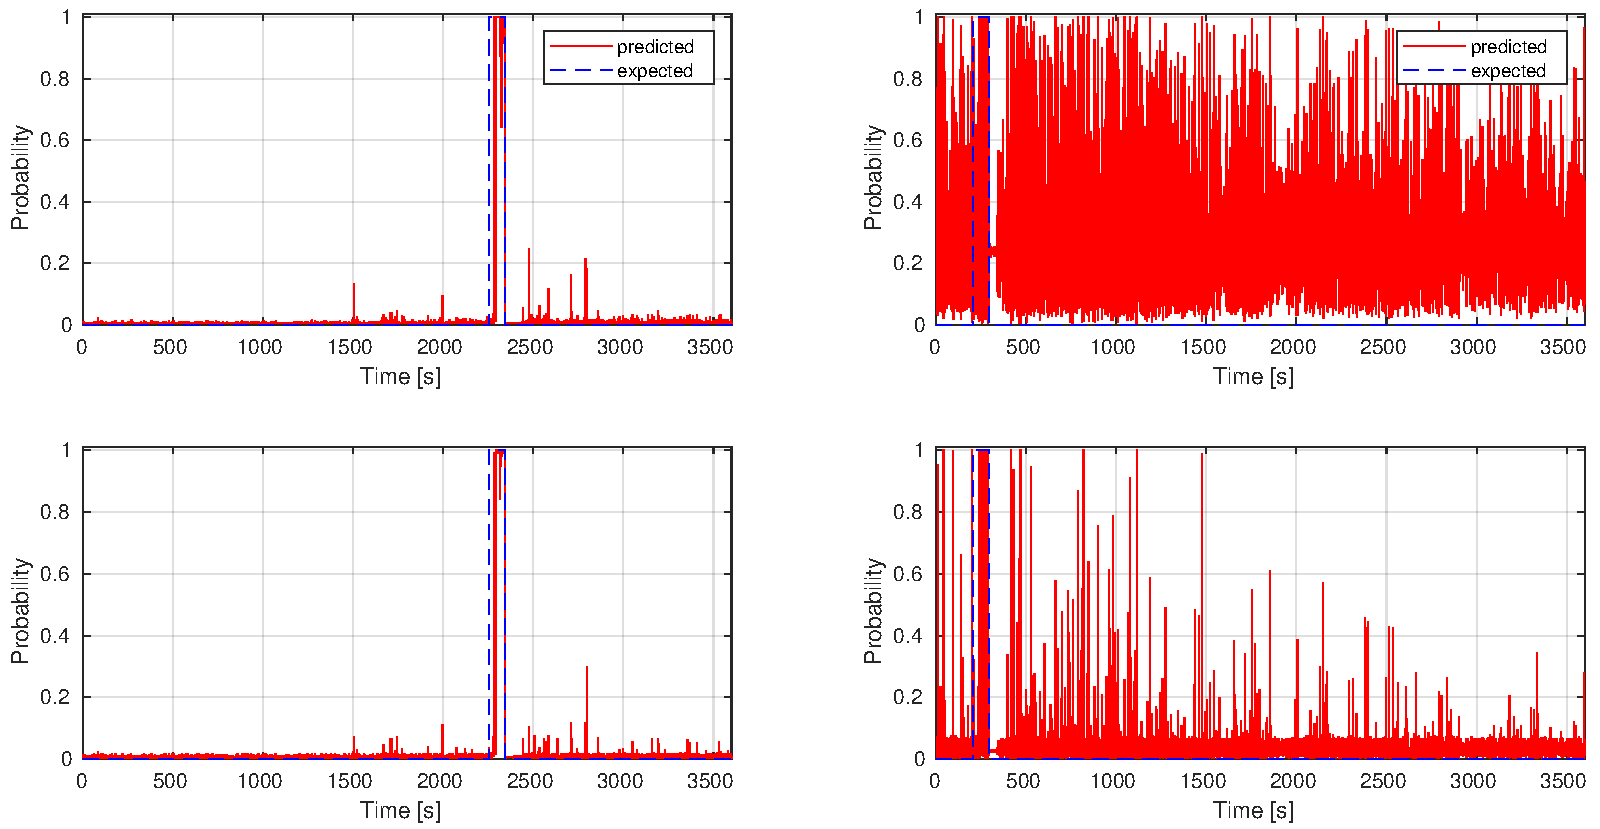
\includegraphics{./plots/nn_fir_4_hidden_512_400_300_150_20_1_10000_30000.pdf}}
	\end{center}
	\caption{2 experiments for 4 hidden layers multilayer perceptron. On the left network adjustment, on the right test. 512 inputs, number of nodes in 4 hidden layers 400, 300, 150, 20. Number of epochs in the particular raw is 10000 and 30000 consecutively.}

	\label{fig:nn_fir_4_hidden_512_400_300_150_20_1_10000_30000}
\end{figure}
\begingroup
\renewcommand{\cleardoublepage}{}
\renewcommand{\clearpage}{}
\chapter{Postprocessing}
\endgroup
Taking into account already explored methods with several different neural network configurations, the best choice seems to be the synergy between raw \verb|iEEG| signals and 4 layers feedforward, especially with higher numer of nodes. The last step in seizure detection is postprocessing. In the experiments chapter about detection basing on raw data, seizures were correctly detected, however with many jump's within ictal period. The seizure nature is that they usually last for several seconds and it is less likely that next seizure will occur right after the previous one with a few seconds gap between both. That knowledge can be exploited in the postprocessing part.
When two neural network seizure predictions occur right after the next one it is more often than not it is still the same seizure. From the other hand if neural network detect seizure in the very one second, most likely it is a false alarm. Therefore when neural network hint the seizure in the particular moment, postprocessing algorithm explores several following samples and checks if the seizure was once again detected. If so a couple of seconds between two detection are treated as one seizure. And at the second extreme, if next detection is absent it means false alarm. Following listing shows \verb|MATLAB| postprocessing implementation for 1 hour predicted data. If prediction is about to be treated as correct seizure, next prediction has to occur within 10 nearest samples. Otherwise it is a false alarm. The biggest drawback of this method is the fact that introduces artificial delay of 10 seconds. 

\begin{lstlisting}[style=custommatlab,frame=single]
postprocessed=zeros(size(prediction));
i=1;
while i<=3600
    if prediction(i,1) >= 0.5
        for j=1:10
            if prediction(i+j,1) >= 0.5
                postprocessed(i:i+j,1)=1;
                break;
            end
        end
        i=i+j;
    else
        i=i+1;
    end
end
\end{lstlisting}

 The postprocessing for the last 2 experiments from \figurename{} \ref{fig:nn_raw_4_hidden_512_400__250_30_1_5000_150000_20000} and \figurename{} \ref{fig:nn_raw_4_hidden_512_400__250_30_1_5000_150000_20000_zoomed}, that is 15000 and 20000 epochs is presented on the \figurename{} \ref{fig:post_nn_raw_4_hidden_512_400__250_30_1_150000_20000.pdf}. The best achieved detection is late around 30 seconds.
\begin{figure}[H]
	\begin{center}
		\scalebox{.57}{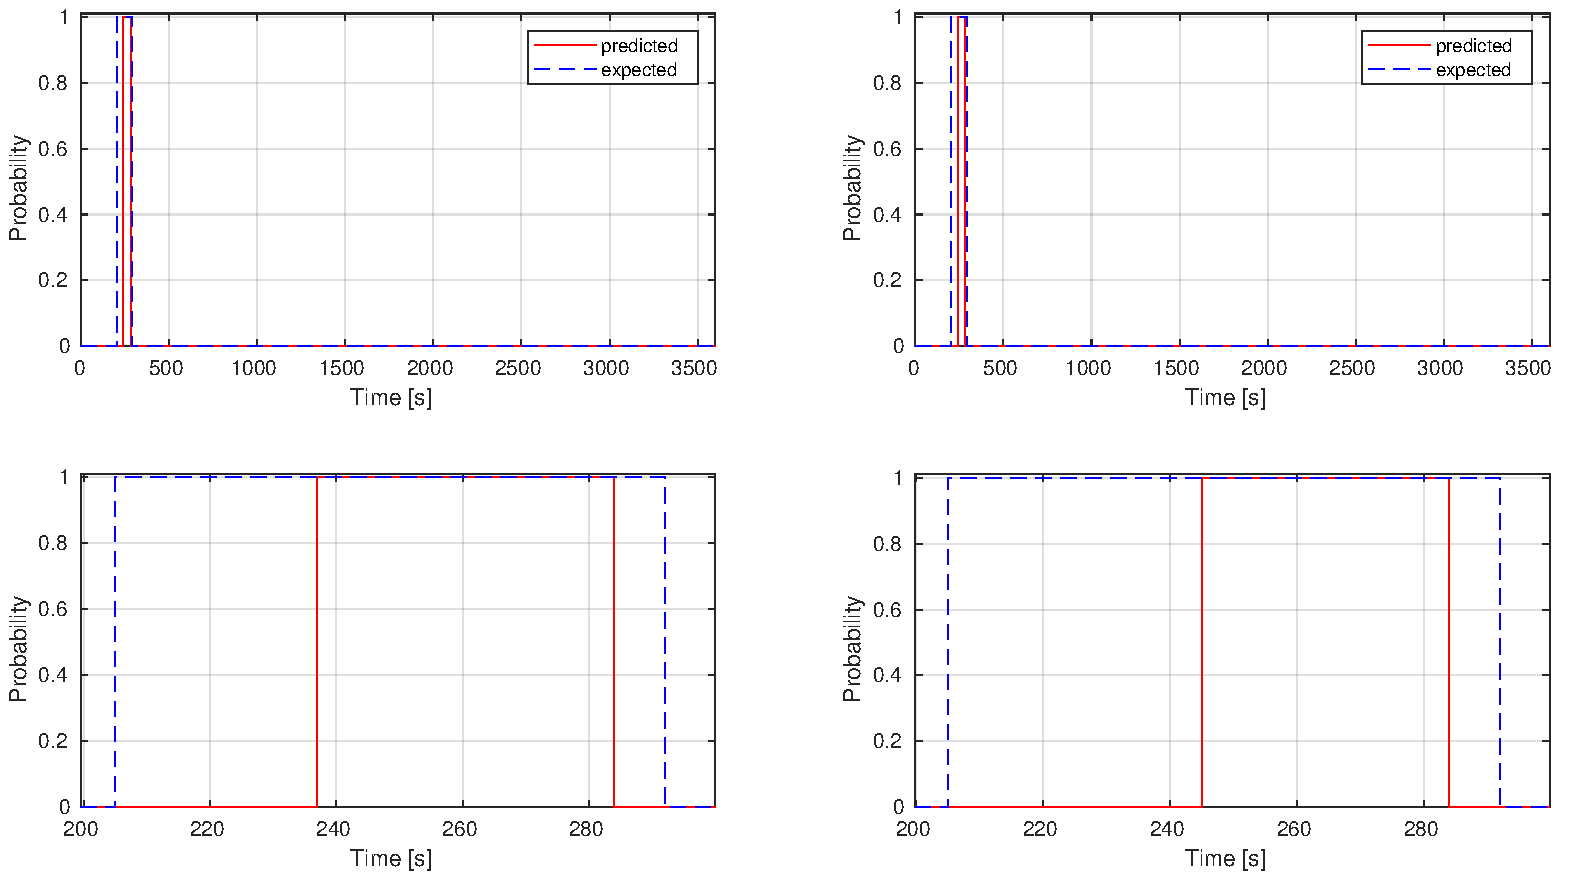
\includegraphics{./plots/post_nn_raw_4_hidden_512_400__250_30_1_150000_20000.pdf}}
	\end{center}
	\caption{Post processed 4 hidden layers neural network prediction, for 15000 and 20000 epochs. Nodes amount 512, 400, 250 and 30. Prediction is 8 seconds faster for 15000 epochs.}

	\label{fig:post_nn_raw_4_hidden_512_400__250_30_1_150000_20000.pdf}
\end{figure}

\begingroup
\renewcommand{\cleardoublepage}{}
\renewcommand{\clearpage}{}
\chapter{Conclusions}
\endgroup
Several methods of epilepsy detection basing on intracranial electroencephalography and machine learning have been discussed. Local binary patterns gave remarkably poor results in the opposite to what was accomplished by several scientist. Finite impulse response filters are not the best option for \verb|iEEG| signal processing. They flatten signals, causing bigger resemblance between ictal and interictal periods. The best technique could be to take an advantage of variability of the signals and expose the differences between adjacent samples. In spite of the lack of successful in \verb|LBP| exploitation, which bases on the differences between adjacent samples, derivative utilisation can expose that differences, for example as a part of proportional-derivative-integral \verb|PID| regulator. Nevertheless there is a success in the detection basing on raw signals. After postprocessing it is clearly visible where the seizure occurred, although with substantial delay.
The fact that only one electrode was utilised for the detection could have significant influence for neural network performance. In addition the amount of epochs, layers and nodes in the particular layers was chosen empirically, even randomly. That quantities as well as the network itself should be chosen according to the problem which they will trying to solve. There is a broad space for enhancement for the presented system, with more electrodes as well as different kinds of neural network utilisation, like convolutional neural networks used extensively in computer vision \cite{convolutional}. 
\begin{appendices}

\begingroup
\renewcommand{\cleardoublepage}{}
\renewcommand{\clearpage}{}
\chapter{Back propagation} \label{ch:back}
\endgroup
The following appendix shows an implementation of the one hidden layer feed forward back propagation algorithm. Without high level libraries, just pure \verb|Python3|. The difficulties in algorithm implementation grow with the number of layers, because back propagation bases on the gradient calculation, where particular gradient in the layer depends on many factors in the following layers. Thus, for the need of the project back propagation was outsourced to the \verb|Tensorflow|/
\section{Output layer}
\begin{minted}[frame=single, linenos]{python}
def gradientsOutput(self, inputs, dedo, w, dActivationFunction, acti_arg1):
    """
    @param inputs, The outputs of the last hidden layer
    @param dedo,   Error gradient with respect to the output
    @param w,      An array of weights between output and the 
                   hidden layer. Is constant
    @param dActivationFunction in the case of this layer is 
                   dSigmoid 
    @param acti_arg1 Argument for dActivationFunction. In this case
                   an output of the last layer
    """
    outputs_length = len(w[0])
    inputs_length = len(w)

    dedw = [[0 for o in range(outputs_length)] for i in range(inputs_length)]
    dedb = [0 for o in range(outputs_length)]
    for o in range(0, outputs_length): 
        for i in range(0, inputs_length):
            dedw[i][o] = dedo[o] * dActivationFunction(acti_arg1[o])*inputs[i]
        
        dedb[o] = dedo[o] * dActivationFunction(acti_arg1[o]) * 1
    return dedw, dedb
\end{minted}
\section{Hidden layer}
\begin{minted}[frame=single, linenos]{python}
def gradients(self, inputs, dedo, w, w2, dActivationFunction, acti_arg1, 
    dActivationFunction_2, acti_arg1_2):
    """
    @param inputs, The input of the nn
    @param dedo,   Error gradient with respect to the output
    @param w,      An array of weights between input and the 
                   hidden layer. Is constant
    @param w2,     An array of weights between hidden layer
                   and the output. Gradient of w depends on them.
                   Is constant
    @param dActivationFunction activation for the hidden layer
    @param acti_arg1 Argument for dActivationFunction. If ReLU then
           should be net inputs z.
    @param dActivationFunction2 activation for the output layer
    @param acti_arg2 Argument for dActivationFunction2. 
    """
    outputs_length = len(w[0]) # of w!
    inputs_length = len(w)

    dedw = [[0 for o in range(outputs_length)] for i in range(inputs_length)]
    dedb = [0 for o in range(outputs_length)]
    
    dedohw = [[0 for o in range(outputs_length)] for i in range(inputs_length)]
    dedohb = [0 for o in range(outputs_length)]
    
    outputs_length2 = len(w2[0])
    inputs_length2 = len(w2)

    for o2 in range(0, outputs_length2):
        dEdActiv = dedo[o2] * dActivationFunction_2(acti_arg1_2[o2])
        for o in range(0, outputs_length):
            dedoh = dEdActiv * w2[o][o2]
            for i in range(0, inputs_length):
                dedohw[i][o] += dedoh
            
            dedohb[o] += dedoh

    for o in range(0, outputs_length):
        dActiv = dActivationFunction(acti_arg1[o])
        for i in range(0, inputs_length):
            dedw[i][o] = dedohw[i][o] * dActiv * inputs[i]
        
        dedb[o] = dedohb[o] * dActiv * 1

    return dedw, dedb
\end{minted}
\section{Back propagation chain}
\begin{minted}[frame=single, linenos]{python}
def learn(self, x, y_desired):
    y = self.think(x)
    dedo = self.dSqe(y, y_desired)

    (dedw2, dedb2) = self.gradientsOutput(self.l1_output, dedo, self.w2, 
        self.dSigmoid, self.output)
    (dedw1, dedb1) = self.gradients(x, dedo, self.w1, self.w2, 
        self.dReLU, self.l1_z, self.dSigmoid, self.output)
    
    self.update(self.w2, self.b2, dedw2, dedb2)
    self.update(self.w1, self.b1, dedw1, dedb1)
\end{minted}

\section{Update function}
\begin{minted}[frame=single, linenos]{python}
def update(self, w, b, dedw, dedb):
    outputs_length = len(w[0])
    inputs_length = len(w)
    
    for o in range(0, outputs_length):
        for i in range(0, inputs_length):
            w[i][o] += dedw[i][o] * self.lr
        
        b[o] += dedb[o] * self.lr
\end{minted}

\end{appendices}
	
	\bibliographystyle{unsrt}
    \bibliography{bibliography}
	
	\listoffigures

	%\begingroup
	%\let\clearpage\relax
	%\listoftables
	%\endgroup

\end{document}

